\chapter{Concepts of Operation for Command and Control}
\label{cha:c2conops}
\newcommand{\HOLcTwoDrulesDate}{06 October 2012}
\newcommand{\HOLcTwoDrulesTime}{17:44}
\begin{SaveVerbatim}{HOLcTwoDrulesTheoremsAlternateControlRepsKeyOne}
\HOLTokenTurnstile{} (\HOLFreeVar{M},\HOLFreeVar{Oi},\HOLFreeVar{Os}) sat \HOLFreeVar{R\sb{\mathrm{2}}} controls \HOLFreeVar{s} andf \HOLFreeVar{R\sb{\mathrm{3}}} controls \HOLFreeVar{s} \HOLTokenImp{}
   (\HOLFreeVar{M},\HOLFreeVar{Oi},\HOLFreeVar{Os}) sat \HOLFreeVar{CA\sb{\mathrm{1}}} controls \HOLFreeVar{Kca\sb{\mathrm{2}}} speaks_for \HOLFreeVar{CA\sb{\mathrm{2}}} \HOLTokenImp{}
   (\HOLFreeVar{M},\HOLFreeVar{Oi},\HOLFreeVar{Os}) sat \HOLFreeVar{CA\sb{\mathrm{2}}} controls \HOLFreeVar{Kp\sb{\mathrm{1}}} speaks_for \HOLFreeVar{P\sb{\mathrm{1}}} \HOLTokenImp{}
   (\HOLFreeVar{M},\HOLFreeVar{Oi},\HOLFreeVar{Os}) sat \HOLFreeVar{CA\sb{\mathrm{2}}} controls \HOLFreeVar{Kp\sb{\mathrm{2}}} speaks_for \HOLFreeVar{P\sb{\mathrm{2}}} \HOLTokenImp{}
   (\HOLFreeVar{M},\HOLFreeVar{Oi},\HOLFreeVar{Os}) sat \HOLFreeVar{R\sb{\mathrm{1}}} controls reps \HOLFreeVar{P\sb{\mathrm{2}}} \HOLFreeVar{R\sb{\mathrm{2}}} \HOLFreeVar{s} \HOLTokenImp{}
   (\HOLFreeVar{M},\HOLFreeVar{Oi},\HOLFreeVar{Os}) sat \HOLFreeVar{Kca\sb{\mathrm{1}}} speaks_for \HOLFreeVar{CA\sb{\mathrm{1}}} \HOLTokenImp{}
   (\HOLFreeVar{M},\HOLFreeVar{Oi},\HOLFreeVar{Os}) sat reps \HOLFreeVar{P\sb{\mathrm{1}}} \HOLFreeVar{R\sb{\mathrm{1}}} (reps \HOLFreeVar{P\sb{\mathrm{2}}} \HOLFreeVar{R\sb{\mathrm{2}}} \HOLFreeVar{s}) \HOLTokenImp{}
   (\HOLFreeVar{M},\HOLFreeVar{Oi},\HOLFreeVar{Os}) sat \HOLFreeVar{Kp\sb{\mathrm{2}}} quoting \HOLFreeVar{R\sb{\mathrm{2}}} says \HOLFreeVar{s} \HOLTokenImp{}
   (\HOLFreeVar{M},\HOLFreeVar{Oi},\HOLFreeVar{Os}) sat \HOLFreeVar{Kca\sb{\mathrm{1}}} says \HOLFreeVar{Kca\sb{\mathrm{2}}} speaks_for \HOLFreeVar{CA\sb{\mathrm{2}}} \HOLTokenImp{}
   (\HOLFreeVar{M},\HOLFreeVar{Oi},\HOLFreeVar{Os}) sat \HOLFreeVar{Kca\sb{\mathrm{2}}} says \HOLFreeVar{Kp\sb{\mathrm{1}}} speaks_for \HOLFreeVar{P\sb{\mathrm{1}}} \HOLTokenImp{}
   (\HOLFreeVar{M},\HOLFreeVar{Oi},\HOLFreeVar{Os}) sat \HOLFreeVar{Kca\sb{\mathrm{2}}} says \HOLFreeVar{Kp\sb{\mathrm{2}}} speaks_for \HOLFreeVar{P\sb{\mathrm{2}}} \HOLTokenImp{}
   (\HOLFreeVar{M},\HOLFreeVar{Oi},\HOLFreeVar{Os}) sat \HOLFreeVar{Kp\sb{\mathrm{1}}} quoting \HOLFreeVar{R\sb{\mathrm{1}}} says reps \HOLFreeVar{P\sb{\mathrm{2}}} \HOLFreeVar{R\sb{\mathrm{2}}} \HOLFreeVar{s} \HOLTokenImp{}
   (\HOLFreeVar{M},\HOLFreeVar{Oi},\HOLFreeVar{Os}) sat \HOLFreeVar{s}
\end{SaveVerbatim}
\newcommand{\HOLcTwoDrulesTheoremsAlternateControlRepsKeyOne}{\UseVerbatim{HOLcTwoDrulesTheoremsAlternateControlRepsKeyOne}}
\begin{SaveVerbatim}{HOLcTwoDrulesTheoremsAlternateControlsOne}
\HOLTokenTurnstile{} (\HOLFreeVar{M},\HOLFreeVar{Oi},\HOLFreeVar{Os}) sat \HOLFreeVar{P\sb{\mathrm{1}}} controls \HOLFreeVar{s\sb{\mathrm{1}}} andf \HOLFreeVar{P\sb{\mathrm{2}}} controls \HOLFreeVar{s\sb{\mathrm{1}}} \HOLTokenImp{}
   (\HOLFreeVar{M},\HOLFreeVar{Oi},\HOLFreeVar{Os}) sat \HOLFreeVar{P\sb{\mathrm{1}}} says \HOLFreeVar{s\sb{\mathrm{1}}} \HOLTokenImp{}
   (\HOLFreeVar{M},\HOLFreeVar{Oi},\HOLFreeVar{Os}) sat \HOLFreeVar{s\sb{\mathrm{1}}}
\end{SaveVerbatim}
\newcommand{\HOLcTwoDrulesTheoremsAlternateControlsOne}{\UseVerbatim{HOLcTwoDrulesTheoremsAlternateControlsOne}}
\begin{SaveVerbatim}{HOLcTwoDrulesTheoremsAlternateControlsTwo}
\HOLTokenTurnstile{} (\HOLFreeVar{M},\HOLFreeVar{Oi},\HOLFreeVar{Os}) sat \HOLFreeVar{P\sb{\mathrm{1}}} controls \HOLFreeVar{s\sb{\mathrm{1}}} andf \HOLFreeVar{P\sb{\mathrm{2}}} controls \HOLFreeVar{s\sb{\mathrm{1}}} \HOLTokenImp{}
   (\HOLFreeVar{M},\HOLFreeVar{Oi},\HOLFreeVar{Os}) sat \HOLFreeVar{P\sb{\mathrm{2}}} says \HOLFreeVar{s\sb{\mathrm{1}}} \HOLTokenImp{}
   (\HOLFreeVar{M},\HOLFreeVar{Oi},\HOLFreeVar{Os}) sat \HOLFreeVar{s\sb{\mathrm{1}}}
\end{SaveVerbatim}
\newcommand{\HOLcTwoDrulesTheoremsAlternateControlsTwo}{\UseVerbatim{HOLcTwoDrulesTheoremsAlternateControlsTwo}}
\begin{SaveVerbatim}{HOLcTwoDrulesTheoremsAlternateControlsRepsOne}
\HOLTokenTurnstile{} (\HOLFreeVar{M},\HOLFreeVar{Oi},\HOLFreeVar{Os}) sat \HOLFreeVar{R\sb{\mathrm{1}}} controls \HOLFreeVar{s} andf \HOLFreeVar{R\sb{\mathrm{2}}} controls \HOLFreeVar{s} \HOLTokenImp{}
   (\HOLFreeVar{M},\HOLFreeVar{Oi},\HOLFreeVar{Os}) sat \HOLFreeVar{P\sb{\mathrm{1}}} quoting \HOLFreeVar{R\sb{\mathrm{1}}} says \HOLFreeVar{s} \HOLTokenImp{}
   (\HOLFreeVar{M},\HOLFreeVar{Oi},\HOLFreeVar{Os}) sat reps \HOLFreeVar{P\sb{\mathrm{1}}} \HOLFreeVar{R\sb{\mathrm{1}}} \HOLFreeVar{s} \HOLTokenImp{}
   (\HOLFreeVar{M},\HOLFreeVar{Oi},\HOLFreeVar{Os}) sat \HOLFreeVar{s}
\end{SaveVerbatim}
\newcommand{\HOLcTwoDrulesTheoremsAlternateControlsRepsOne}{\UseVerbatim{HOLcTwoDrulesTheoremsAlternateControlsRepsOne}}
\begin{SaveVerbatim}{HOLcTwoDrulesTheoremsAlternateControlsRepsTwo}
\HOLTokenTurnstile{} (\HOLFreeVar{M},\HOLFreeVar{Oi},\HOLFreeVar{Os}) sat \HOLFreeVar{R\sb{\mathrm{1}}} controls \HOLFreeVar{s} andf \HOLFreeVar{R\sb{\mathrm{2}}} controls \HOLFreeVar{s} \HOLTokenImp{}
   (\HOLFreeVar{M},\HOLFreeVar{Oi},\HOLFreeVar{Os}) sat \HOLFreeVar{P\sb{\mathrm{2}}} quoting \HOLFreeVar{R\sb{\mathrm{2}}} says \HOLFreeVar{s} \HOLTokenImp{}
   (\HOLFreeVar{M},\HOLFreeVar{Oi},\HOLFreeVar{Os}) sat reps \HOLFreeVar{P\sb{\mathrm{2}}} \HOLFreeVar{R\sb{\mathrm{2}}} \HOLFreeVar{s} \HOLTokenImp{}
   (\HOLFreeVar{M},\HOLFreeVar{Oi},\HOLFreeVar{Os}) sat \HOLFreeVar{s}
\end{SaveVerbatim}
\newcommand{\HOLcTwoDrulesTheoremsAlternateControlsRepsTwo}{\UseVerbatim{HOLcTwoDrulesTheoremsAlternateControlsRepsTwo}}
\begin{SaveVerbatim}{HOLcTwoDrulesTheoremsDelegates}
\HOLTokenTurnstile{} \HOLTokenForall{}\HOLBoundVar{P\sb{\mathrm{2}}} \HOLBoundVar{R\sb{\mathrm{2}}} \HOLBoundVar{M} \HOLBoundVar{Oi} \HOLBoundVar{Os} \HOLBoundVar{P\sb{\mathrm{1}}} \HOLBoundVar{R\sb{\mathrm{1}}} \HOLBoundVar{s\sb{\mathrm{1}}} \HOLBoundVar{s\sb{\mathrm{2}}}.
     (\HOLBoundVar{M},\HOLBoundVar{Oi},\HOLBoundVar{Os}) sat \HOLBoundVar{R\sb{\mathrm{1}}} controls \HOLBoundVar{s\sb{\mathrm{1}}} \HOLTokenImp{}
     (\HOLBoundVar{M},\HOLBoundVar{Oi},\HOLBoundVar{Os}) sat \HOLBoundVar{P\sb{\mathrm{1}}} quoting \HOLBoundVar{R\sb{\mathrm{1}}} says \HOLBoundVar{s\sb{\mathrm{1}}} \HOLTokenImp{}
     (\HOLBoundVar{M},\HOLBoundVar{Oi},\HOLBoundVar{Os}) sat reps \HOLBoundVar{P\sb{\mathrm{1}}} \HOLBoundVar{R\sb{\mathrm{1}}} \HOLBoundVar{s\sb{\mathrm{1}}} \HOLTokenImp{}
     (\HOLBoundVar{M},\HOLBoundVar{Oi},\HOLBoundVar{Os}) sat \HOLBoundVar{s\sb{\mathrm{1}}} impf \HOLBoundVar{s\sb{\mathrm{2}}} \HOLTokenImp{}
     (\HOLBoundVar{M},\HOLBoundVar{Oi},\HOLBoundVar{Os}) sat \HOLBoundVar{P\sb{\mathrm{2}}} quoting \HOLBoundVar{R\sb{\mathrm{2}}} says \HOLBoundVar{s\sb{\mathrm{2}}}
\end{SaveVerbatim}
\newcommand{\HOLcTwoDrulesTheoremsDelegates}{\UseVerbatim{HOLcTwoDrulesTheoremsDelegates}}
\begin{SaveVerbatim}{HOLcTwoDrulesTheoremsDirect}
\HOLTokenTurnstile{} \HOLTokenForall{}\HOLBoundVar{P\sb{\mathrm{2}}} \HOLBoundVar{M} \HOLBoundVar{Oi} \HOLBoundVar{Os} \HOLBoundVar{P\sb{\mathrm{1}}} \HOLBoundVar{s\sb{\mathrm{1}}} \HOLBoundVar{s\sb{\mathrm{2}}}.
     (\HOLBoundVar{M},\HOLBoundVar{Oi},\HOLBoundVar{Os}) sat \HOLBoundVar{P\sb{\mathrm{1}}} controls \HOLBoundVar{s\sb{\mathrm{1}}} \HOLTokenImp{}
     (\HOLBoundVar{M},\HOLBoundVar{Oi},\HOLBoundVar{Os}) sat \HOLBoundVar{P\sb{\mathrm{1}}} says \HOLBoundVar{s\sb{\mathrm{1}}} \HOLTokenImp{}
     (\HOLBoundVar{M},\HOLBoundVar{Oi},\HOLBoundVar{Os}) sat \HOLBoundVar{s\sb{\mathrm{1}}} impf \HOLBoundVar{s\sb{\mathrm{2}}} \HOLTokenImp{}
     (\HOLBoundVar{M},\HOLBoundVar{Oi},\HOLBoundVar{Os}) sat \HOLBoundVar{P\sb{\mathrm{2}}} says \HOLBoundVar{s\sb{\mathrm{2}}}
\end{SaveVerbatim}
\newcommand{\HOLcTwoDrulesTheoremsDirect}{\UseVerbatim{HOLcTwoDrulesTheoremsDirect}}
\begin{SaveVerbatim}{HOLcTwoDrulesTheoremsDual}
\HOLTokenTurnstile{} \HOLTokenForall{}\HOLBoundVar{P\sb{\mathrm{3}}} \HOLBoundVar{M} \HOLBoundVar{Oi} \HOLBoundVar{Os} \HOLBoundVar{P\sb{\mathrm{1}}} \HOLBoundVar{P\sb{\mathrm{2}}} \HOLBoundVar{s\sb{\mathrm{1}}} \HOLBoundVar{s\sb{\mathrm{3}}}.
     (\HOLBoundVar{M},\HOLBoundVar{Oi},\HOLBoundVar{Os}) sat \HOLBoundVar{P\sb{\mathrm{1}}} meet \HOLBoundVar{P\sb{\mathrm{2}}} controls \HOLBoundVar{s\sb{\mathrm{1}}} \HOLTokenImp{}
     (\HOLBoundVar{M},\HOLBoundVar{Oi},\HOLBoundVar{Os}) sat \HOLBoundVar{P\sb{\mathrm{1}}} says \HOLBoundVar{s\sb{\mathrm{1}}} \HOLTokenImp{}
     (\HOLBoundVar{M},\HOLBoundVar{Oi},\HOLBoundVar{Os}) sat \HOLBoundVar{P\sb{\mathrm{2}}} says \HOLBoundVar{s\sb{\mathrm{1}}} \HOLTokenImp{}
     (\HOLBoundVar{M},\HOLBoundVar{Oi},\HOLBoundVar{Os}) sat \HOLBoundVar{s\sb{\mathrm{1}}} impf \HOLBoundVar{s\sb{\mathrm{3}}} \HOLTokenImp{}
     (\HOLBoundVar{M},\HOLBoundVar{Oi},\HOLBoundVar{Os}) sat \HOLBoundVar{P\sb{\mathrm{3}}} says \HOLBoundVar{s\sb{\mathrm{3}}}
\end{SaveVerbatim}
\newcommand{\HOLcTwoDrulesTheoremsDual}{\UseVerbatim{HOLcTwoDrulesTheoremsDual}}
\begin{SaveVerbatim}{HOLcTwoDrulesTheoremsDualControl}
\HOLTokenTurnstile{} (\HOLFreeVar{M},\HOLFreeVar{Oi},\HOLFreeVar{Os}) sat \HOLFreeVar{P\sb{\mathrm{1}}} meet \HOLFreeVar{P\sb{\mathrm{2}}} controls \HOLFreeVar{s} \HOLTokenImp{}
   (\HOLFreeVar{M},\HOLFreeVar{Oi},\HOLFreeVar{Os}) sat \HOLFreeVar{P\sb{\mathrm{1}}} says \HOLFreeVar{s} \HOLTokenImp{}
   (\HOLFreeVar{M},\HOLFreeVar{Oi},\HOLFreeVar{Os}) sat \HOLFreeVar{P\sb{\mathrm{2}}} says \HOLFreeVar{s} \HOLTokenImp{}
   (\HOLFreeVar{M},\HOLFreeVar{Oi},\HOLFreeVar{Os}) sat \HOLFreeVar{s}
\end{SaveVerbatim}
\newcommand{\HOLcTwoDrulesTheoremsDualControl}{\UseVerbatim{HOLcTwoDrulesTheoremsDualControl}}
\begin{SaveVerbatim}{HOLcTwoDrulesTheoremsDualReps}
\HOLTokenTurnstile{} (\HOLFreeVar{M},\HOLFreeVar{Oi},\HOLFreeVar{Os}) sat \HOLFreeVar{R\sb{\mathrm{1}}} meet \HOLFreeVar{R\sb{\mathrm{2}}} controls \HOLFreeVar{s} \HOLTokenImp{}
   (\HOLFreeVar{M},\HOLFreeVar{Oi},\HOLFreeVar{Os}) sat \HOLFreeVar{P\sb{\mathrm{1}}} quoting \HOLFreeVar{R\sb{\mathrm{1}}} says \HOLFreeVar{s} \HOLTokenImp{}
   (\HOLFreeVar{M},\HOLFreeVar{Oi},\HOLFreeVar{Os}) sat \HOLFreeVar{P\sb{\mathrm{2}}} quoting \HOLFreeVar{R\sb{\mathrm{2}}} says \HOLFreeVar{s} \HOLTokenImp{}
   (\HOLFreeVar{M},\HOLFreeVar{Oi},\HOLFreeVar{Os}) sat reps \HOLFreeVar{P\sb{\mathrm{1}}} \HOLFreeVar{R\sb{\mathrm{1}}} \HOLFreeVar{s} \HOLTokenImp{}
   (\HOLFreeVar{M},\HOLFreeVar{Oi},\HOLFreeVar{Os}) sat reps \HOLFreeVar{P\sb{\mathrm{2}}} \HOLFreeVar{R\sb{\mathrm{2}}} \HOLFreeVar{s} \HOLTokenImp{}
   (\HOLFreeVar{M},\HOLFreeVar{Oi},\HOLFreeVar{Os}) sat \HOLFreeVar{s}
\end{SaveVerbatim}
\newcommand{\HOLcTwoDrulesTheoremsDualReps}{\UseVerbatim{HOLcTwoDrulesTheoremsDualReps}}
\begin{SaveVerbatim}{HOLcTwoDrulesTheoremsToken}
\HOLTokenTurnstile{} \HOLTokenForall{}\HOLBoundVar{P\sb{\mathrm{2}}} \HOLBoundVar{M} \HOLBoundVar{Oi} \HOLBoundVar{Os} \HOLBoundVar{K\sb{\mathrm{1}}} \HOLBoundVar{P\sb{\mathrm{1}}} \HOLBoundVar{s\sb{\mathrm{1}}} \HOLBoundVar{s\sb{\mathrm{2}}}.
     (\HOLBoundVar{M},\HOLBoundVar{Oi},\HOLBoundVar{Os}) sat \HOLBoundVar{P\sb{\mathrm{1}}} controls \HOLBoundVar{s\sb{\mathrm{1}}} \HOLTokenImp{}
     (\HOLBoundVar{M},\HOLBoundVar{Oi},\HOLBoundVar{Os}) sat \HOLBoundVar{K\sb{\mathrm{1}}} says \HOLBoundVar{s\sb{\mathrm{1}}} \HOLTokenImp{}
     (\HOLBoundVar{M},\HOLBoundVar{Oi},\HOLBoundVar{Os}) sat \HOLBoundVar{K\sb{\mathrm{1}}} speaks_for \HOLBoundVar{P\sb{\mathrm{1}}} \HOLTokenImp{}
     (\HOLBoundVar{M},\HOLBoundVar{Oi},\HOLBoundVar{Os}) sat \HOLBoundVar{s\sb{\mathrm{1}}} impf \HOLBoundVar{s\sb{\mathrm{2}}} \HOLTokenImp{}
     (\HOLBoundVar{M},\HOLBoundVar{Oi},\HOLBoundVar{Os}) sat \HOLBoundVar{P\sb{\mathrm{2}}} says \HOLBoundVar{s\sb{\mathrm{2}}}
\end{SaveVerbatim}
\newcommand{\HOLcTwoDrulesTheoremsToken}{\UseVerbatim{HOLcTwoDrulesTheoremsToken}}
\newcommand{\HOLcTwoDrulesTheorems}{
\HOLThmTag{c2Drules}{AlternateControlRepsKey1}\HOLcTwoDrulesTheoremsAlternateControlRepsKeyOne
\HOLThmTag{c2Drules}{AlternateControls1}\HOLcTwoDrulesTheoremsAlternateControlsOne
\HOLThmTag{c2Drules}{AlternateControls2}\HOLcTwoDrulesTheoremsAlternateControlsTwo
\HOLThmTag{c2Drules}{AlternateControlsReps1}\HOLcTwoDrulesTheoremsAlternateControlsRepsOne
\HOLThmTag{c2Drules}{AlternateControlsReps2}\HOLcTwoDrulesTheoremsAlternateControlsRepsTwo
\HOLThmTag{c2Drules}{Delegates}\HOLcTwoDrulesTheoremsDelegates
\HOLThmTag{c2Drules}{Direct}\HOLcTwoDrulesTheoremsDirect
\HOLThmTag{c2Drules}{Dual}\HOLcTwoDrulesTheoremsDual
\HOLThmTag{c2Drules}{DualControl}\HOLcTwoDrulesTheoremsDualControl
\HOLThmTag{c2Drules}{DualReps}\HOLcTwoDrulesTheoremsDualReps
\HOLThmTag{c2Drules}{Token}\HOLcTwoDrulesTheoremsToken
}

% \section{Introduction}
% \label{sec:introduction}

% \subsection{Objectives}
% \label{sec:objectives}

% \section{Background}
% \label{sec:background}

Computer-enabled command and control is used often in command and
control of high-value commercial transactions, remotely piloted
aircraft, strategic ballistic missiles, and cyber operations. In
operations depending on computer-enabled command and control,
integrity of command and control (C2) is \emph{everything}.  Imagine
if operators questioned whether their weapons would work
correctly. Imagine if people doubted the integrity or authenticity of
the orders they received. Operations would grind to a halt because
people receiving orders would not believe anything they were told and
commanders issuing orders would have no confidence that their orders
would be obeyed.

In this chapter, we introduce the notions of power as a \emph{center
  of gravity} and \emph{trust as center of gravity}. Power and trust
are motivators for a rigorous assessment of trustworthiness. To make
these notions concrete, we illustrate a rigorous development process
around an example command and control scenario.

\section{Centers of Gravity, Critical Capabilities, and Critical
  Requirements}

\begin{figure}[t]
  \centering
  \begin{tabular}{cc}
    \begin{minipage}{0.48\linewidth}
      \centering{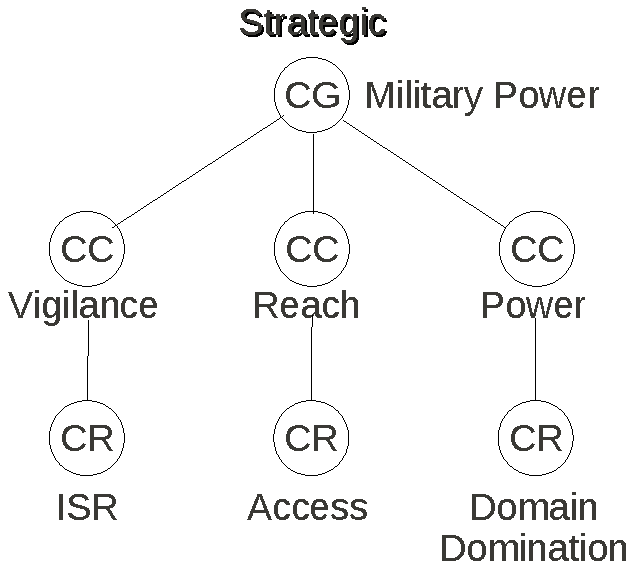
\includegraphics[width=0.6\linewidth]{Figures/c2conops/milPowerCOG}}
    \end{minipage}
    &
    \begin{minipage}{0.48\linewidth}
     \centering{ 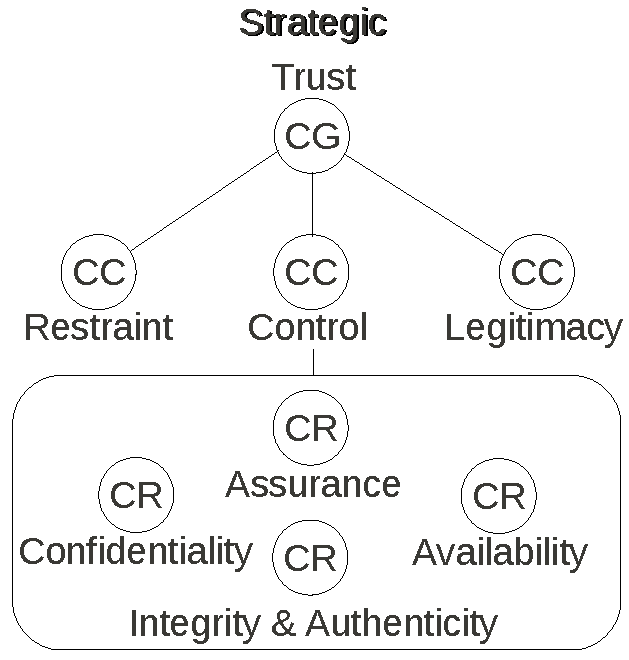
\includegraphics[width=0.6\linewidth]{Figures/c2conops/trustCOG}}\\
   \end{minipage}\\
   (a) Military Power as a Center of Gravity & (b) Trust as a Center of Gravity\\
  \end{tabular}
  \caption{Military Power and Trust Centers of Gravity}
  \label{fig:cogs}
\end{figure}

Centers of gravity (CGs) are the \emph{primary sources of moral or
  physical strength, power and resistance}.  CGs are \emph{hubs of all
  power}.  In war, a strategic objective is to destroy or neutralize
an adversary's center of gravity.  By so doing, the adversary is
\emph{dislocated}, i.e., thrown off balance, so that their ability to
operate quickly, decisively, precisely, and effectively degraded.

Centers of gravity emerge from a collection of primary abilities known
as \emph{critical capabilities} in the context of a given mission or
scenario.  For example, the combined capabilities of ground, air, and
space surveillance contribute the the critical capability of
\emph{global vigilance} that is one of three critical capabilities
that form the basis for military capability as a center of gravity---a
hub of power. The other two capabilities are global reach (the ability
to access any part of the globe) and global power (the ability to
dominate anywhere in the globe).

Another center of gravity is \emph{trust}.  Trust and trustworthiness
are both the glue that holds systems together as well as the oil that
keeps them running smoothly.  Without trust, systems freeze. What
happens when you are driving and a warning light signals your engine
or brakes are malfunctioning? If you are like most people, you pull
over as soon as possible and stop.

In military systems, there are three critical capabilities that
constitute trust as a center of gravity.
\begin{enumerate}
\item Restraint: the ability to exercise appropriate self-control, in
  this case the ability to react with appropriate proportionality,
\item Legitimacy: the acceptance of the actions taken because they are
  viewed to be appropriate in light of the situation, and
\item Control: the ability to command and control forces and systems
  with complete integrity, accuracy, and accountability.
\end{enumerate}
Figure~\ref{fig:cogs}(a) shows military power as a center of gravity
and its critical capabilities and requirements. In an environment
heavily dependent on computer-enabled communications, command and
control, and intelligence (C3I), the trustworthiness of the
computational infrastructure in terms of hardware, software, networks,
and protocols is essential, as is the trustworthiness of the access
control employed from control of physical memory up to and including
information flow policies. Thus, \emph{trust} as a strategic center of
gravity is alongside military power as a center of gravity.

% \paragraph{Assurance of Integrity and Authenticity}

Figure~\ref{fig:cogs}(b) shows trust as a center of gravity along with
the critical capability of \emph{control}. Positive control of forces
requires assurance of confidentiality, availability, and integrity and
authenticity. Imagine if people could not believe the information or
the orders they received. They would be dislocated and
paralyzed. Given the criticality of integrity and authenticity, it is
essential that the highest degree of precision and accuracy of
understanding combined with the highest degree of assurance of
integrity and authenticity be provided to critical missions.  This is
the motivation for using the access-control logic combined with formal
verification with theorem provers such as HOL.  As everything is fully
disclosed and nothing is left to the imagination, assurance and
conceptual unity is achieved.

% Your task this week is to devise and verify using the access-control
% logic \cite{ACST} and its implementation in HOL \cite{HOL}, a command
% and control CONOPS for \emph{launching} or \emph{aborting} an action
% that involves operations in cyberspace. Examples include pure
% cyberspace operations such as disabling a specific computer or
% network, the release of information damaging to an adversary, to the
% kinetic world of launching remotely piloted aircraft and/or releasing
% weapons.

% Our objective is to devise operations and assure their integrity of
% and \emph{the logic behind them using HOL} within the specific
% assumptions on recognized authorities, authenticated commands,
% certifications, roles, delegations, and jurisdictions. The benefits of
% formal verification in HOL (or any trustworthy computer-assisted
% reasoning tool) are (1) \emph{assurance} of logical correctness, (2)
% \emph{full disclosure} of all definitions and assumptions, (3)
% \emph{rapid evaluation, certification, and reuse} by third parties,
% (4) \emph{enhanced conceptual unity} due to clarity and precision, and
% (5) \emph{enhanced confidence in achieving mission objectives} due to
% assurance.

% This sets a new standard for design, verification, and assurance in
% cyber operations.  Please take extra care to do the best possible job
% as your reports and HOL code for this week's problem will be used as
% evidence of how you are able to achieve assurance of cyber operations
% with mathematical rigor to external reviewers of our program.

% \subsection{Deliverables}
% \label{sec:deliverables}

% This week you will deliver the following:
% \begin{enumerate}
% \item A full written report in the format expected in your Cyber
%   Engineering Seminar: Cover Page, Executive Summary, Problem
%   Statement, Background, Assumptions, Techniques and Tools, Problem
%   Solution, Risk Assessment, and Bibliography.
% \item Complete verification of your CONOPS in HOL using the
%   access-control logic.
% \item Your written report will include appendices giving the contents
%   of your theories and your source code.
% \item You will deliver electronic copies of your source code and
%   reports within the \textbf{subdirectory structure I have
%     provided}. By so doing, I can check your work by executing
%   \texttt{Holmake} in the subdirectory you send me.
% \end{enumerate}
% You may use the text, figures, tables, and my HOL source code
% \textbf{\redtext{with attribution}}. If you collaborated over ideas,
% please note that in your report and your source code. Make sure you
% include your name on the title page of your report.

\section{Representing Concepts of Operations in the Access-Control
  Logic}
\label{sec:conops}

\begin{center}
  \fbox{\begin{minipage}[h]{0.8\linewidth} Definition of
      \textbf{Concept of Operations}: JP 5-0, Joint Operation Planning
      \begin{small}
        \begin{quote}
          \emph{ ``The CONOPS clearly and concisely expresses what [is
            to be] accomplish[ed] and how it will be done using
            available resources. It describes how the actions of
            $\ldots$ components and supporting organizations will be
            integrated, synchronized, and phased to accomplish the
            mission $\ldots$''}
        \end{quote}
      \end{small}
    \end{minipage}}
\end{center}

% The command and control scenario presented in
% Section~\ref{sec:c2-scenario}, is a specific instance of how we can
% use the access-control logic to formally describe and justify the
% logic behind a \emph{concept of operations} (CONOPS). In this section
% we briefly describe the principles of describing CONOPS in the
% logic. 

Concepts of operations (CONOPS) in JP 5-0: Joint Operation Planning,
is defined to be a description of the coordination, integration, and
sequencing of actions of components and organizations.  From a command
and control standpoint, we focus on the flow of commands from one
principal to the next (recalling that principals are people, roles,
cryptographic keys, processes, etc.), within a context of policies
that govern actions, jurisdiction of controlling authorities, and
trust assumptions.  Using the access-control logic, each step in a
CONOPS---\emph{a response by a principal corresponding to a component
  in the CONOPS} to a command, request, or statement in conjunction
with policies, jurisdiction of controlling authorities, and trust
assumptions---is a derived inference rule in the logic.

\begin{figure}[tb]
  \centering
  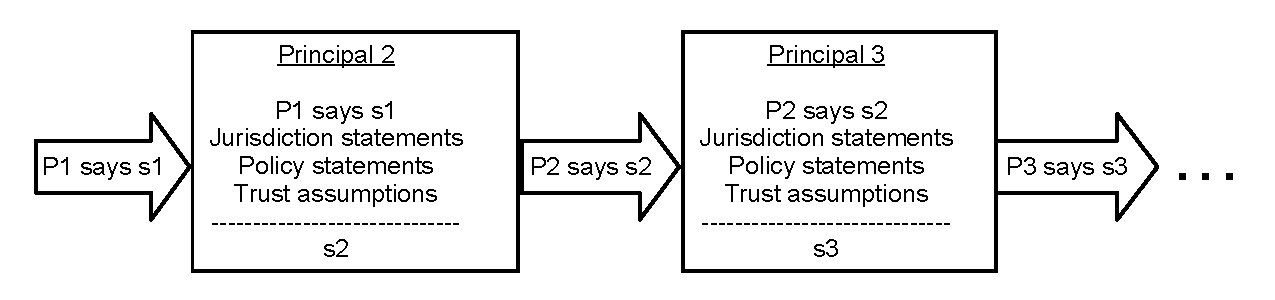
\includegraphics[width=0.95\linewidth]{Figures/c2conops/blockDiagram}
  \caption{Flow of Control in Concepts of Operations}
  \label{fig:conops-flow}
\end{figure}

Figure~\ref{fig:conops-flow} shows the flow of commands in a CONOPS
from left to right starting with principal $P_1$'s command, statement,
or request $P_1 \says s_1$. Principal $P_2$ evaluates $P_1$'s
statement within the context of jurisdiction statements, policy
statements, and trust assumptions.  If $P_2$ concludes $s_2$, then the
next step in the CONOPS, $P_s \says s_2$, is taken. Principal $P_3$
does a similar analysis, and so on down the line until the operation
is complete.

The boxes corresponding to deliberations and actions of principals
$P_2$ and $P_3$ deliberately appear as \emph{derived inference rules
  in the access-control logic}.  Each rule serves as a logical
justification of the actions of a CONOPS component to specific
situations. The advantages of using formally proved inference rules
include: (1) establishing the operating assumptions on which logical
validity is based, (2) assurance and full disclosure due to formal
verification, and (3) conceptual unity, when descriptions and
verifications are done and distributed using computer-assisted
reasoning tools such as HOL.

\begin{figure}[t]
  \centering
  \begin{tabular}{cc}
  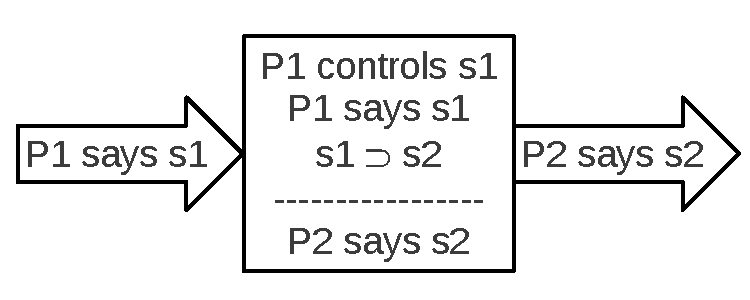
\includegraphics[width=0.4\linewidth]{Figures/c2conops/direct} 
  &
  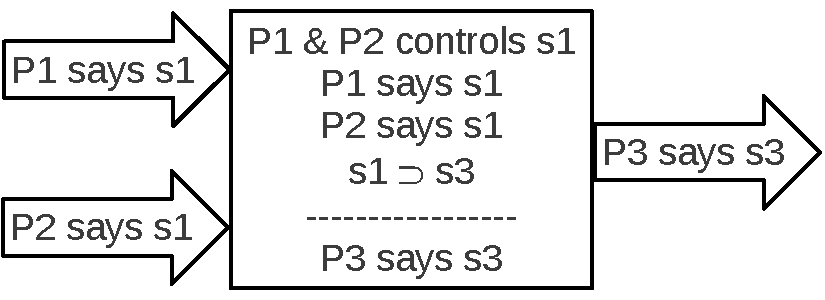
\includegraphics[width=0.4 \linewidth]{Figures/c2conops/dual}\\
  (a) Direct & (b) Dual\\
  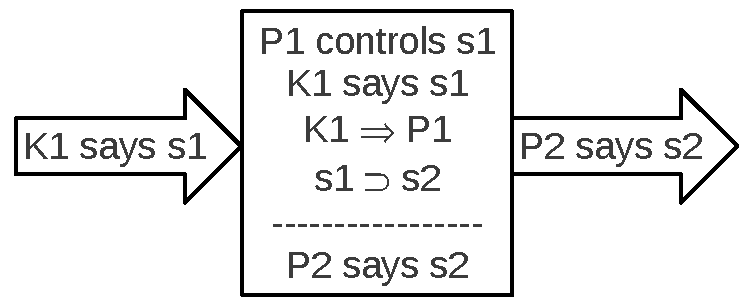
\includegraphics[width=0.4\linewidth]{Figures/c2conops/token} 
  &
  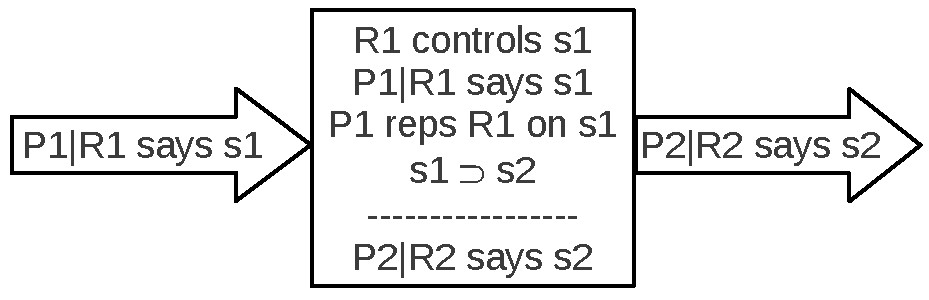
\includegraphics[width=0.4 \linewidth]{Figures/c2conops/roles}\\
  (c) With Tokens & (d) Using Delegates or Relays \\
\end{tabular}
  \caption{Types of Command and Control}
  \label{fig:C2-types}
\end{figure}

When representing a CONOPS, the logic and dependencies upon which the
CONOPS depend are often easiest revealed by putting oneself in the
position of the principal involved at a given step of the CONOPS. The
overall question is what is needed for you as that principal to
execute your part of the CONOPS?  What statements or commands do you
expect to receive? What certificates do you need? What root trust
assumptions are you using, e.g., keys of root certificate authorities?
Who are the authorities you recognize and what is their jurisdiction?
Under what policies are you operating, (for example, if the commander
says \emph{go} then you are to issue the \emph{launch} command)?

When devising CONOPS and representing them in the access-control
logic, the patterns that are illustrated in
Figures~\ref{fig:C2-types}(a) through \ref{fig:C2-types}(d) often are
used in some combination. The arrows going into a box are the
statements or commands received by a principal in a CONOPS. The arrow
going out of a box is the statement or command issued by a principal
in a CONOPS. Inside a box is the derived inference rule in the
access-control logic justifying the statement or command issued by a
principal in a CONOPS. Notice that each rule depends on more than the
received command or statement. Internal to each box are assumptions
consisting of jurisdiction (control) statements, trust assumptions
(e.g., $K_1 \speaksfor P_1$), and policy statements (e.g., $s_1
\implies s_2$). These internal assumptions are the \emph{operational
  mode} or \emph{state} of a principal in a CONOPS.

In the sections that follow, for each case we give an informal
description, a simple template in the form of a derived inference
rule, and the equivalent HOL theorem showing the validity of the
derived rule.

\subsection{Direct Control}
\label{sec:direct-control}

By \emph{direct command and control} we mean that the authority behind
a command and the principal issuing the command are one and the
same. Figure~\ref{fig:C2-types}(a) illustrates this case. The components
of this case are as follows:
\begin{itemize}
\item Input Command: $P_1 \says s_1$
\item Authority and jurisdiction: $P_1 \controls s_1$
\item Policy: $s_1 \implies s_2$
\item Output Command: $P_2 \says s_2$
\end{itemize}


\subsection{Dual Control}
\label{sec:dual-control}

By \emph{dual control} we mean that two principals acting jointly,
i.e., $P_1 \with P_2$, are the authorities behind a command and both
must issue the command. Figure~\ref{fig:C2-types}(b) illustrates this
case. The components of this case are as follows;
\begin{itemize}
\item Input Commands: $P_1 \says s_1$ and $P_2 \says s_1$
\item Authority and jurisdiction: $P_1 \with P_2 \controls s_1$
\item Policy: $s_1 \implies s_3$
\item Output Command: $P_3 \says s_3$
\end{itemize}

\subsection{Tokens}
\label{sec:tokens}

By \emph{token} we mean the use of some token that stands for or
speaks for a principal. Often, this token is a cryptographic key
$K_P$, (authenticated by key certificates or known by trust
assumptions), that speaks for a principal $P$, i.e., $K_P \speaksfor
P$. Figure~\ref{fig:C2-types}(c) illustrates this case. The components
of this case are as follows:
\begin{itemize}
\item Input Command: $K_1 \says s_1$
\item Authority and jurisdiction: $P_1 \controls s_1$
\item Key certificate or trust assumption: $K_1 \speaksfor P_1$
\item Policy: $s_1 \implies s_2$
\item Output Command: $P_2 \says s_2$
\end{itemize}


\subsection{Delegates and Relays}
\label{sec:delegates-relays}

By \emph{delegate or relay} we mean the use of principals acting in a
\emph{role} such as mission commander, or acting as an intermediary
passing on statements or commands, e.g., a messenger. The logical
construct used to express these relationships is the relation
$\reps{P}{Q}{\varphi}$, i.e., $P$ is $Q$'s delegate or representative
on statement $\varphi$. The inference rule in
Figure~\ref{fig:C2-types}(d) is essentially the \emph{Reps} inference
rule with the addition of the policy statement. The components of this
case are as follows:
\begin{itemize}
\item Input Command: $P_1 \quoting R_1 \says s_1$
\item Authority and jurisdiction: $R_1 \controls s_1$
\item Role certificate or trust assumption: $\reps{P_1}{R_1}{s_1}$
\item Policy: $s_1 \implies s_2$
\item Output Command: $P_2 \quoting R_2 \says s_2$
\end{itemize}

What is written above is typical of cases where mission roles are
employed, e.g., \emph{mission commander, operator,} etc. Principals
$P_i$ are assigned to mission roles $R_i$. When acting in those roles,
principals $P_i$ acting in roles $R_i$ make statements of the form
$P_i \quoting R_i \says s_i$. Authentication of people acting in roles
is done in the usual way via certified statements or by trust
assumptions.

\begin{exercise}[\synthesis]
\label{exercise:direct}
  \begin{enumerate}[{A.}]
  \item Using the access-control logic, prove the derived inference
    rule corresponding to direct control.
  \item Using HOL, prove the theorem corresponding to the
    access-control logic inference rule for direct control.
  \item Using HOL, devise an ML function that is an inference rule
    (i.e., returns a theorem corresponding to the output command when
    applied to the input command theorem, authority/jurisdiction
    theorem, and policy theorem) based on the HOL theorem for direct
    control.
  \end{enumerate}
\end{exercise}

\begin{exercise}[\synthesis]
  \begin{enumerate}[{A.}]
  \item Using the access-control logic, prove the derived inference
    rule corresponding to dual control.
  \item Using HOL, prove the theorem corresponding to the
    access-control logic inference rule for dual control.
  \item Using HOL, devise an ML function that is an inference rule
    (i.e., returns a theorem corresponding to the output command when
    applied to the input command theorems, authority/jurisdiction
    theorem, and policy theorem) based on the HOL theorem for dual
    control.
  \end{enumerate}
\end{exercise}

\begin{exercise}[\synthesis]
  \begin{enumerate}[{A.}]
  \item Using the access-control logic, prove the derived inference
    rule corresponding to token control.
  \item Using HOL, prove the theorem corresponding to the
    access-control logic inference rule for token control.
  \item Using HOL, devise an ML function that is an inference rule
    (i.e., returns a theorem corresponding to the output command when
    applied to the input command theorems, authority/jurisdiction
    theorem, and policy theorem) based on the HOL theorem for token
    control.
  \end{enumerate}
\end{exercise}

\begin{exercise}[\synthesis]
  \begin{enumerate}[{A.}]
  \item Using the access-control logic, prove the derived inference
    rule corresponding to delegate control.
  \item Using HOL, prove the theorem corresponding to the
    access-control logic inference rule for delegate control.
  \item Using HOL, devise an ML function that is an inference rule
    (i.e., returns a theorem corresponding to the output command when
    applied to the input command theorems, authority/jurisdiction
    theorem, and policy theorem) based on the HOL theorem for delegate
    control.
  \end{enumerate}
\end{exercise}

% In the next section, we develop the high-level CONOPS for the scenario
% introduced in Section~\ref{sec:c2-scenario}.
% In the three sections that follow, we give three views of the CONOPS
% created to satisfy the flow of command and control and certificate
% authority hierarchy shown in
% Figure~\ref{fig:ca-hierarchy-c2-flow}. Section~\ref{sec:refinement1}
% gives a high-level description of CONOPS using only the mission roles
% of Blue Forces Commander, Blue Forces Operator, Gold Forces Commander,
% Gold Forces Operator, and the
% Weapon. Section~\ref{sec:conops-with-staff} refines the high-level
% CONOPS description by adding people assigned to mission
% roles. Section~\ref{sec:conops-with-keys} is the final refinement that
% adds cryptographic keys to the flow of control along with certificate
% authority hierarchy in Figure~\ref{fig:ca-hierarchy-c2-flow}(a).


\section{A Command and Control Scenario}
\label{sec:c2-scenario}

% \subsection{Problem Statement}
% \label{sec:problem}

Our scenario is one that requires the exercise of joint authority in
the midst of an established trust infrastructure.  This is typical of
joint operations or coalition operations.  The specifics of what is
being controlled are unimportant. It could be a remotely piloted
vehicle; it could be the launch of an air-to-ground missile; it could
be the launch of a strategic nuclear ballistic missile; it could be
the transfer of hundreds of millions of dollars between two banks.

Our scenario has two forces operating jointly: \emph{Blue Forces} and
\emph{Gold Forces}.  Each force has its own command structure:
\emph{Blue Command} and \emph{Gold Command}. The mission for which we
are designing and assuring a cyber command and control (C2)
infrastructure is described below.
\begin{enumerate}
\item \textbf{Oversight and jurisdiction}: Blue and Gold Commanders
  have joint control over a mission involving the \emph{launching} of
  a weapon.  Both Blue and Gold Commanders have two mission commands:
  \texttt{go} and \texttt{nogo}. For the mission to proceed, a person
  in the role of Blue Commander and a person operating in the role
  Gold Commander must both issue the \texttt{go} command for the
  mission to proceed.
\item \textbf{Operators}: people who are authorized as Blue or Gold Operators
  ultimately issue the command to the weapon under joint control. The
  agreed-upon policy is the same for both Blue and Gold Operators:
  each Operator will issue the \texttt{launch} command when he or she
  receives an authenticated \texttt{go} command from their respective
  commander, e.g., the Gold Operator will issue the \texttt{launch}
  command to the weapon when his/her Gold Commander issues the
  \texttt{go} command. The corresponding policy holds for the Blue
  Operator.  Similarly, if the Blue or Gold Operator receives a
  \texttt{nogo} order from their respective Commanders, the Operator
  will issue an \texttt{abort} command to the weapon.
\item \textbf{Weapon}: the weapon has two commands: \texttt{launch} and
  \texttt{abort}. \texttt{Launch} activates and deploys the
  weapon. \texttt{Abort} puts the weapon in safe mode and returns the
  weapon to its initial standby state. The policy the weapon is
  designed to operate within is this: (1) the weapon can only be
  launched if it receives an authenticated \texttt{launch} command
  from both the Blue Operator and Gold Operator, and (2) either the
  Blue Operator or Gold Operator can \texttt{abort} the mission
  without the others \texttt{abort} command.
\end{enumerate}

Our goal is to describe Blue Operator, Gold Operator, and weapon
operations in terms of \emph{derived inference rules in the
  access-control logic} that are \emph{formally verified in
  HOL}. These operations will include the expected commands received,
policies, assumptions about jurisdiction and authority, necessary
certifications, and trust assumptions.

% \subsection{Assumptions}
% \label{sec:assumptions}

We assume the infrastructure supporting the operation includes the
following:
\begin{enumerate}
\item a hierarchy of certificate authorities to authenticate
  cryptographic keys, provide attribution for messages, and
  authenticate mission roles;
\item a root of trust for cryptographic keys, i.e., the public key
  for the Joint Forces Certificate Authority, $K_{JFCA}$ will be
  distributed in a secure manner to Commanders, Operators, and weapons
  prior to the mission start;
\item established mission roles in terms of what commands each role
  controls;
\item formally defined mission commands and weapon commands.
\end{enumerate}

\paragraph*{Certificate Authority Hierarchy}
\begin{figure}[t]
  \centering
  \begin{tabular}[t]{cc}
    \begin{minipage}{0.48\linewidth}
      % \begin{figure}[t]
      \centering
      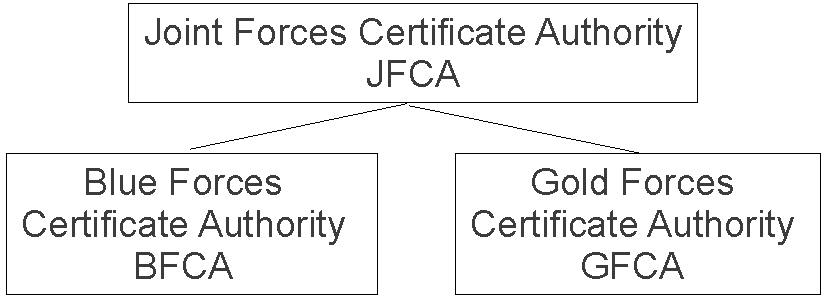
\includegraphics[width=0.95\linewidth]{Figures/c2conops/CAHierarchy}
      % \caption{Certificate Authority Hierarchy}
      % \label{fig:ca-hierarchy}
      % \end{figure}
    \end{minipage}
    &
    \begin{minipage}{0.48\linewidth}
      % \begin{figure}[t]
      \centering
      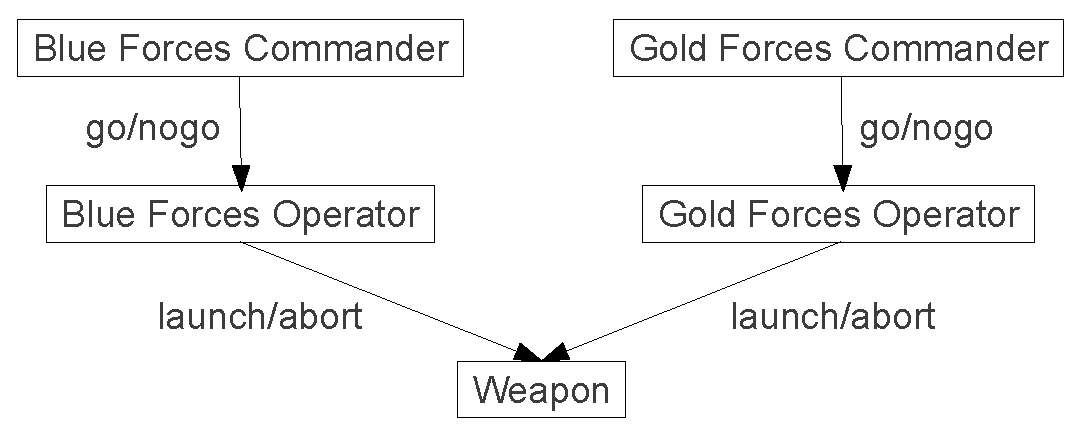
\includegraphics[width=0.95\linewidth]{Figures/c2conops/conops}
      % \caption{Flow of Command and Control}
      % \label{fig:c2-flow}
      % \end{figure}
    \end{minipage}\\
    (a) Certificate Authority Hierarchy & (b) Flow of Command and Control\\
  \end{tabular}
  
  \caption{Certificate Authority Hierarchy and Flow of Command and Control}
\label{fig:ca-hierarchy-c2-flow}
\end{figure}

Figure~\ref{fig:ca-hierarchy-c2-flow}(a) shows the relationships among
the Joint Forces Certificate Authority (JFCA), Blue Forces Certificate
Authority (BFCA), and Gold Forces Certificate Authority (GFCA).  The
primary purpose of the JFCA is to authenticate the BFCA and GFCA for
specific missions.  Note, it could very well be the case that each
joint forces mission has a different JFCA.  This prevents mission
creep in terms of authorizations for one mission leaking over to
separate missions.

The BFCA and GFCA are anticipated to be the CAs normally recognized by
Blue and Gold Forces, respectively.  There is no need for cross
recognition of BFCAs or GFCAs independently of the JFCA.  This is
consistent with the intent of establishing JFCAs on a
mission-by-mission basis.

\begin{table}[tb]
  \centering
  \begin{center}
  \begin{footnotesize}
    \begin{tabular}[h]{|r| >{$}c<{$}|l|}
      \hline
      \textbf{Certificate Authority} &\textbf{Associated Key} & \textbf{How Authenticated}\\
      \hline
      JFCA & K_{JFCA} & Pre-distributed to all mission principals\\
      Blue Forces CA & K_{BFCA} & Authenticated by JFCA\\
      Gold Forces CA & K_{GFCA} & Authenticated by JFCA\\
      \hline
    \end{tabular}
  \end{footnotesize}
\end{center}
\caption{Mission Certificate Authorities, Keys, and Authentication}
\label{tab:mission-ca}
\end{table}

Table~\ref{tab:mission-ca} defines the keys associated with each
certificate authority and who authenticates a particular CA.  We see
that keys for the Blue and Gold Forces CAs are authenticated by the
Joint Forces CA. The JFCA's key $K_{JFCA}$ is a trust assumption and
is assumed to have been distributed in a secure fashion prior to the
mission to all mission principals.

We represent the information in Table~\ref{tab:mission-ca} in the
access-control logic as follows.
\begin{align*}
  \text{Trust Assumption: } & K_{JFCA} \speaksfor \text{JFCA}\\
  \text{Jurisdiction of JFCA: } & JFCA \controls (K_{BFCA} \speaksfor \text{BFCA})\\
 \text{BFCA certificate signed by JFCA: } & K_{JFCA} \says (K_{BFCA} \speaksfor \text{BFCA})\\
  \text{Jurisdiction of JFCA: } & JFCA \controls (K_{GFCA} \speaksfor \text{GFCA})\\
 \text{BFCA certificate signed by JFCA: } & K_{JFCA} \says (K_{GFCA} \speaksfor \text{GFCA})
\end{align*}
The starting trust assumption is $K_{JFCA} \speaksfor \text{JFCA}$,
which implies that key $K_{JFCA}$ has been distributed prior to the
mission. Both \emph{controls} statements reflect the authority of JFCA
over the Blue and Gold Forces CAs.  Both \emph{says} statements are
the key certificates signed by JFCA using $K_{JFCA}$.

\begin{table}[t]
  \centering
  \begin{center}
  \begin{footnotesize}
    \begin{tabular}[h]{|r| >{$}c<{$}|l|}
      \hline
      \textbf{Role} & \textbf{Commands} & \textbf{How Authenticated}\\
      \hline
      Blue Forces Commander & \texttt{go}/\texttt{nogo} & Pre-distributed to all Blue Forces mission principals\\
      Gold Forces Commander & \texttt{go}/\texttt{nogo} & Pre-distributed to all Gold Forces mission principals\\
      Blue Forces Operator & \texttt{launch}/\texttt{abort} & Blue Forces Commander\\
      Gold Forces Operator & \texttt{launch}/\texttt{abort} & Gold Forces Commander\\
      \hline
    \end{tabular}
  \end{footnotesize}
\end{center}

\caption{Mission Roles, Commands, and Authentication}
\label{tab:mission-roles}
\end{table}

\paragraph*{Mission Commands and Weapon Commands}
The mission is initiated with a \texttt{go} command; it is aborted
with a \texttt{nogo} command. Mission commands are defined as follows.
\begin{gather*}
  missionCommands \isa go \ora nogo.
\end{gather*}
Weapon commands are defined as follows.
\begin{gather*}
  weaponCommands \isa launch \ora abort.
\end{gather*}
The flow of command and control is shown in Figure~\ref{fig:ca-hierarchy-c2-flow}.

\paragraph*{Mission Roles and Jurisdiction}

Table~\ref{tab:mission-roles} associates commands each mission role
can make and who authenticates personnel to act in each role. For
example, both Blue and Gold Forces Commanders can issue \texttt{go} or
\texttt{nogo} commands, which are received by Blue and Gold Forces
Operators.  Blue and Gold Forces Operators can issue \texttt{launch}
and \texttt{abort} commands to weapons.

The information in Table~\ref{tab:mission-roles} is best thought of in
the context of each mission role---specifically, what orders a
principal receives while acting in a role and the conditions under
which the orders are obeyed.

\subparagraph*{Blue and Gold Forces Operators}

The Blue and Gold Forces Operators receive \texttt{go/nogo} commands
from the Blue and Gold Forces Commanders, respectively. Operators, as
a result of receiving these commands within the operational context
and policies under which they function, issue \texttt{launch} or
\texttt{abort} commands to the weapon.  We develop the details of the
operational context and policies for Operators as follows.

The recognition by operators of their commanders' authority over
\texttt{go/nogo} commands is given below as trust
assumptions. Specifically, Blue Force Operators recognize the
authority of Blue Force Commanders and Gold Force Operators recognize
the authority of Gold Force Commanders.
\begin{enumerate}[{}]
\item \emph{Operational Context for Blue Force Operators:}
\begin{align*}
  \text{Trust Assumption: } & BFC \controls \action{\mathtt{go}}\\
  \text{Trust Assumption: } & BFC \controls \action{\mathtt{nogo}}
\end{align*}
\item \emph{Operational Context for Gold Force Operators:}
\begin{align*}
  \text{Trust Assumption: } & GFC \controls \action{\mathtt{go}}\\
  \text{Trust Assumption: } & GFC \controls \action{\mathtt{nogo}}
\end{align*}

\end{enumerate}

The orders received by Blue Force and Gold Force Operators come from
their respective Commanders.
\begin{enumerate}[{}]
\item \emph{Commands received by Blue Force Operators:}
  \begin{align*}
    \text{Command from Blue Force Commander: } & BFC \says \action{go}\\
    \text{Command from Blue Force Commander: } & BFC \says \action{nogo}
  \end{align*}
\item \emph{Commands received by Gold Force Operators:}
  \begin{align*}
    \text{Command from Gold Force Commander: } & GFC \says \action{go}\\
    \text{Command from Gold Force Commander: } & GFC \says \action{nogo}
  \end{align*}
\end{enumerate}

Given the operational context and commands received by each operator,
both the Blue and Gold Forces Operators are able to conclude
\action{go} or \action{nogo} when their respective Commanders transmit
their orders. This is a result of applying the \emph{Controls}
inference rule.

At this point, Operators can conclude \action{go} or
\action{nogo}. What allows them to conclude $BFO \says
\action{launch}$, $BFO \says \action{abort}$, $GFO \says
\action{launch}$, or $GFO \says \action{abort}$? The implied
\emph{operational policy} for both Operators is
\begin{align*}
  \text{Operational Policy: } & \action{go} \implies \action{launch}\\
  \text{Operational Policy: } & \action{nogo} \implies \action{abort}
\end{align*}

Assuming the above are the operational policies for Blue and Gold
Forces Operators, both Operators can conclude \action{launch} and
\action{abort} using \emph{Modus Ponens} when the appropriate mission
command is issued by their respective Commanders.  

The final step is how do both Operators conclude $BFO \says
\action{launch}$, $BFO \says \action{abort}$, $GFO \says
\action{launch}$, or $GFO \says \action{abort}$ when they have
concluded either \action{launch} or \action{abort}? They do so simply
by using the \emph{Says} inference rule.

% \begin{align*}
%   \text{Jurisdiction of BFC: } & BFC \controls (BFO \controls \action{launch})\\
%   \text{Jurisdiction of BFC: } & BFC \controls (BFO \controls \action{abort})\\
%   \text{Jurisdiction of GFO: } & GFC \controls (GFO \controls \action{launch})\\
%   \text{Jurisdiction of GFO: } & GFC \controls (GFO \controls \action{abort})\\
%   \text{Authentication of BFO: } & BFC \says (BFO \controls \action{launch})\\
%   \text{Authentication of BFO: } & BFC \says (BFO \controls \action{abort})\\
%   \text{Authentication of GFO: } & GFC \says (GFO \controls \action{launch})\\
%   \text{Authentication of GFO: } & GFC \says (GFO \controls \action{abort})\\
% \end{align*}
\paragraph*{Weapons Policy}

Figure~\ref{tab:weapon-launch-abort} shows the command and control
requirements for the weapon to be launched or aborted. \emph{Dual
  control} is required for weapons launch, whereas \emph{single
  control} is all that is required to abort. The weapons policy
expressed in the access-control logic is as follows.
\begin{table}[tb]
  \centering
  \begin{center}
  \begin{tabular}[h]{|r|l|}
    \hline
    \textbf{Action} & \textbf{Command and Control Requirements}\\
    \hline
    Weapons Launch & \emph{Launch} ordered by both Blue and Gold Operators\\
    Weapons Abort & \emph{Abort} ordered by either Blue or Gold Operator\\
    \hline
  \end{tabular}
\end{center}

\caption{Weapon Launch and Abort}
\label{tab:weapon-launch-abort}
\end{table}


The above policy is represented by:
\begin{align*}
\text{Joint Authority of BFO and GFO over launch: } & (BFO \with GFO) \controls \action{launch}\\
\text{BFO jurisdiction over abort: } & BFO \controls \action{abort}\\
\text{GFO jurisdiction over abort: } & GFO \controls \action{abort}
\end{align*}
With the above policies, the Operator commands received by the weapon,
i.e., $BFO \says \action{launch}$, $BFO \says \action{abort}$, $GFO
\says \action{launch}$, or $GFO \says \action{abort}$, and using the
\emph{\& Says} and \emph{Controls} inference rules, the weapon can
derive whether or not to launch or abort.

In the sections that follow, we do four refinements of this scenario,
each with an increasing amount of detail:
\begin{itemize}
\item Refinement 1: CONOPS using only mission roles,
\item Refinement 2: CONOPS with personnel assigned to mission roles,
\item Refinement 3: CONOPS with cryptographic keys associated with
  mission personnel, and
\item Refinement 4: CONOPS with message syntax and semantics.
\end{itemize}


\section{Refinement 1: CONOPS Using Only Mission Roles}
\label{sec:refinement1}

\begin{figure}[t]
  \centering
  \begin{tabular}{cc}
    \begin{minipage}{0.48\linewidth}
      \centering{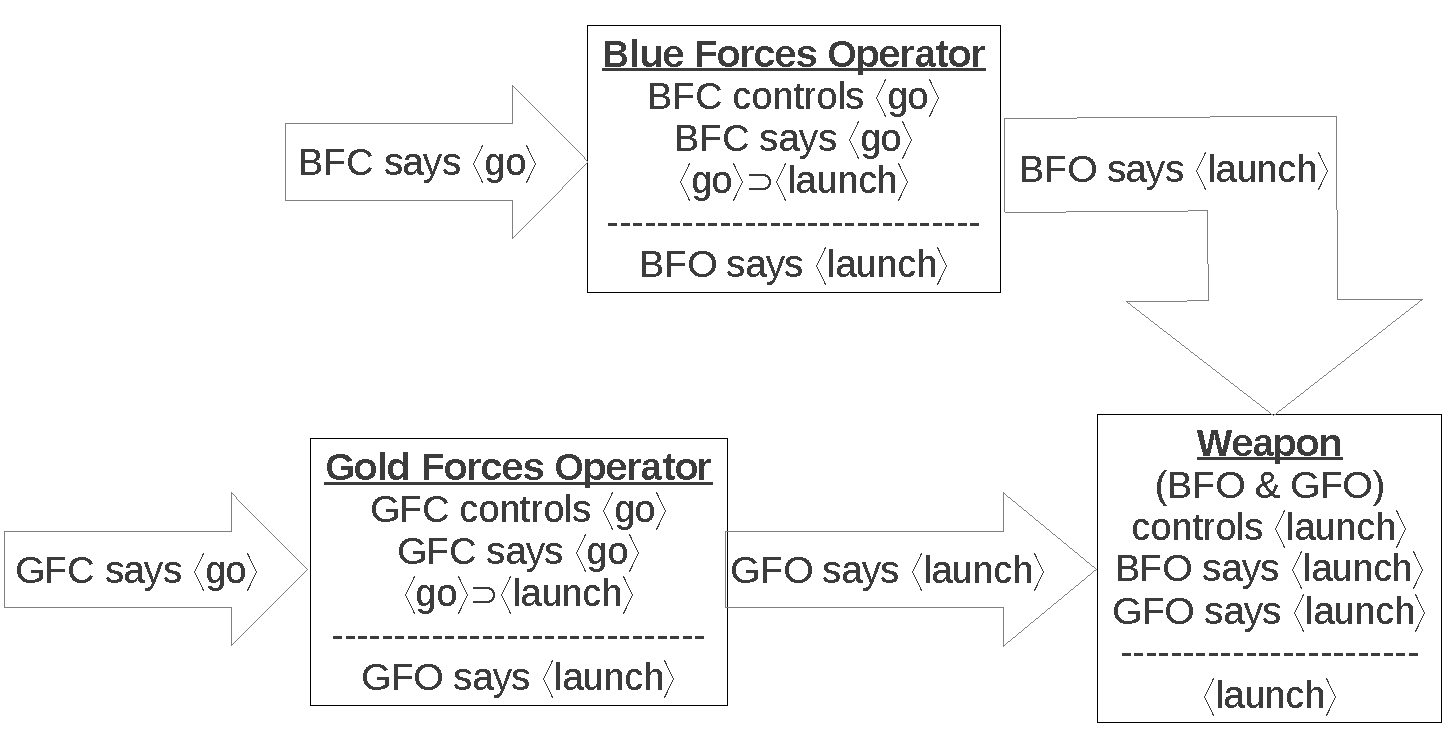
\includegraphics[width=0.95\linewidth]{Figures/c2conops/launchCONOPS}}
    \end{minipage}
    &
    \begin{minipage}{0.48\linewidth}
      \centering{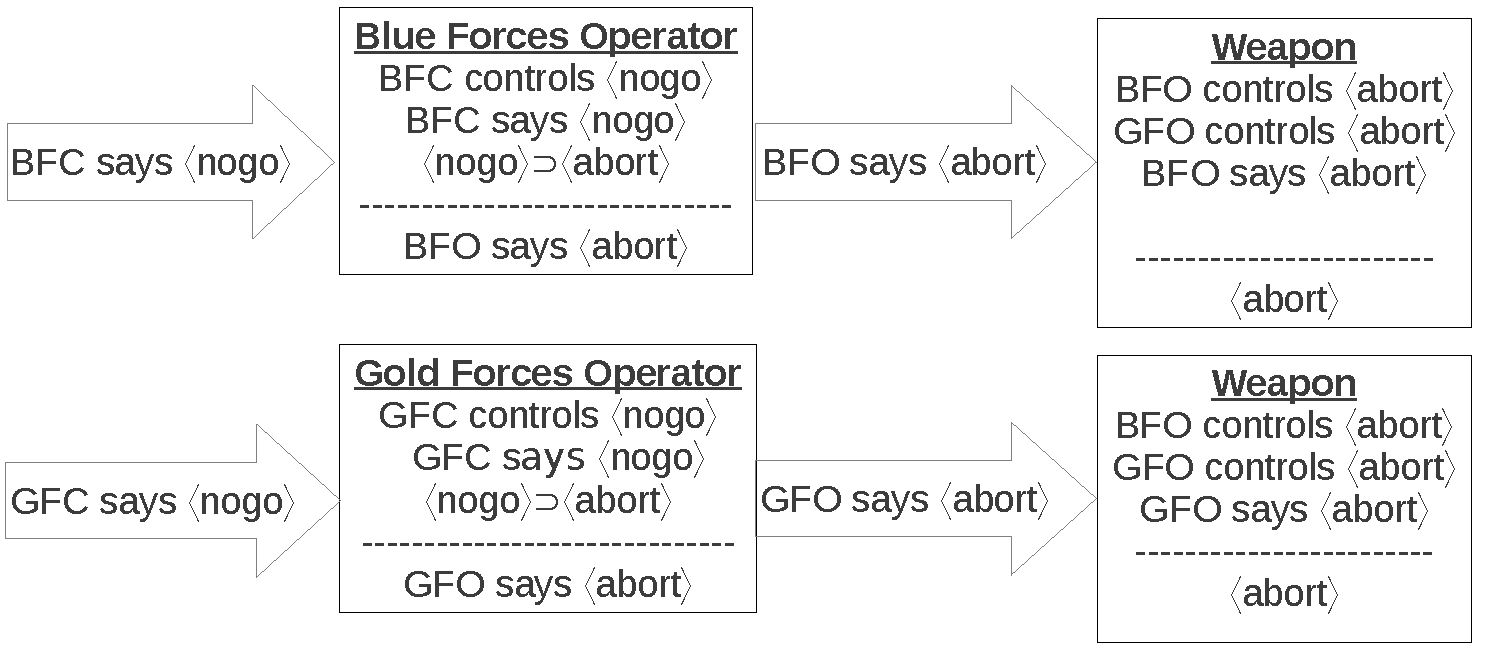
\includegraphics[width=0.95\linewidth]{Figures/c2conops/abortCONOPS}}
    \end{minipage}\\
    (a) Launch CONOPS & (b) Abort CONOPS\\
  \end{tabular}
  \caption{High-Level View of Launch and Abort CONOPS}
  \label{fig:launch-abort-conops}
\end{figure}


% \label{sec:refinement1}

\paragraph*{CONOPS in the Access-Control Logic }


Figures~\ref{fig:launch-abort-conops}(a) and (b) show the high-level
CONOPS for launching or aborting the weapon, respectively. Each box
represents a \emph{derived inference rule} in the access-control
logic. The view is high level because the rules are expressed in terms
of roles only. Details regarding personnel, cryptographic keys, and
necessary certifications are omitted.

Notice that the form of Figures~\ref{fig:launch-abort-conops}(a) and
\ref{fig:launch-abort-conops}(b) correspond to the flow of command and
control as shown in Figure~\ref{fig:ca-hierarchy-c2-flow}(b). The
difference is that Figure~\ref{fig:launch-abort-conops} makes all the
hypotheses and conclusions explicit in the form of derived inference
rules. For example, take the box corresponding to \emph{Blue Forces
  Operator}.  \emph{BFO} receives an order from the Blue Forces
Commander: $BFC \says \action{go}$. The Blue Forces Operator evaluates
$BFC \says \action{go}$ in the context of jurisdiction statements,
policy statements, and trust assumptions.  If the Blue Forces Operator
concludes \action{Launch}, then (using the \emph{Says} rule), the Blue
Forces Operator issues the \emph{Launch} command, i.e., $BFO \says
\action{Launch}$.

Essentially, what we must do based on the informal CONOPS statements
and assumptions is write the jurisdiction statements, policy
statements, and trust assumptions necessary for the Blue Forces
Operator to conclude \emph{Launch} when he/she receives the \emph{go}
command from the Blue Forces Commander. 

\begin{figure}[t]
  \centering
  % \begin{tabular}{c}
  % \begin{minipage}{0.4\linewidth}
  %   \begin{center}
  %     \begin{footnotesize}
  %       \begin{tabular}{|r<{.}>{$}l<{$}l|}
  %         \hline
  %         1 & P \says \varphi_1 & Received command\\
  %         2 & P \controls \varphi_1 & Jurisdiction of P\\
  %         3 & \varphi_1 \implies \varphi_2 & Policy assumption\\
  %         4 & \varphi_1 & 2, 1 Controls\\
  %         5 & \varphi_2 & 4, 3 Modus Ponens\\
  %         6 & Q \says \varphi_2 & 5 Says\\
  %         \hline
  %       \end{tabular}
  %     \end{footnotesize}

  %   \end{center}
  % \end{minipage}
  % \\
  % (a) Proof of Implied Controls with Says \\\\
  \begin{minipage}{1.0\linewidth}
    \begin{center}
      \begin{footnotesize}
        \begin{tabular}{|r<{.}>{$}p{0.45\linewidth}<{$}l|}
          \hline
          1 & P_1 \with P_2 \controls \varphi & Dual control policy\\
          2 & P_1 \says \varphi & Received command\\
          3 & P_2 \says \varphi & Received command\\
          4 & (P_1 \says \varphi) \wedge (P_2 \says \varphi) & 2, 3 Conjunction\\
          5 & (P_1 \says \varphi) \wedge (P_2 \says \varphi) \equiv P \with P_2\says \varphi & \& Says\\
          6 & P_1 \with P_2 \says \varphi & 5, 4 Equivalence\\
          7 & \varphi & 6, 1 Controls\\
          \hline
        \end{tabular}
      \end{footnotesize}
    \end{center}
  \end{minipage}
  \caption{Proof of Dual Control}
  % \label{fig:implied-controls-with-says-proof}
  \label{fig:dual-control}
\end{figure}

\begin{figure}[t]
  \centering
  \begin{tabular}{c}
  \begin{minipage}{0.8\linewidth}
    \begin{center}
      \begin{tabular}{|r<{.}>{$}p{0.45\linewidth}<{$}l|}
        \hline
        1 & P_1 \controls \varphi \wedge P_2 \controls \varphi & assumption\\
        2 & P_1 \says \varphi & assumption\\
        3 & P_1 \controls \varphi & 1 Simplification (1)\\
        4 & \varphi & 3, 2 Controls\\
        \hline
      \end{tabular}
    \end{center}
  \end{minipage}\\
  (a) Proof of Alternate Controls (1) \\
  \\
  \begin{minipage}{0.8\linewidth}
    \begin{center}
      \begin{tabular}{|r<{.}>{$}p{0.45\linewidth}<{$}l|}
        \hline
        1 & P_1 \controls \varphi \wedge P_2 \controls \varphi & assumption\\
        2 & P_2 \says \varphi & assumption\\
        3 & P_2 \controls \varphi & 1 Simplification (2)\\
        4 & \varphi & 3, 2 Controls\\
        \hline
      \end{tabular}
    \end{center}
  \end{minipage}\\
  (b) Proof of Alternate Controls (2)
\end{tabular}
  \caption{Proof of Alternate Controls Rule}
  \label{fig:alternate-controls-proof}
\end{figure}

\subparagraph*{Weapons Launch CONOPS}

The inference rule for the Blue Forces Operator is:
\begin{gather*}
  \irule
  {
    \begin{array}{c}
      BFC \controls \action{go} \quad BFC \says \action{go}\quad
      \action{go} \implies \action{launch}\\
    \end{array}
  }
  {BFO \says \action{launch}}
  {BFO Launch 1}.
\end{gather*}
The launch rule for the Gold Forces Operator has the corresponding
form, i.e.,
\begin{gather*}
  \irule
  {
    \begin{array}{c}
      GFC \controls \action{go} \quad GFC \says \action{go}\quad
      \action{go} \implies \action{launch}\\
    \end{array}
  }
  {GFO \says \action{launch}}
  {GFO Launch 1}.
\end{gather*}
Both Blue and Gold Operators are relying the same inference rule where
principals and commands are parameters:
\begin{gather*}
  \irule
  {
    \begin{array}{c}
      P_1 \controls \varphi_1 \quad P_1 \says \varphi_1\quad
      \varphi_1 \implies \varphi_2\\
    \end{array}
  }
  {P_2 \says \varphi_2}
  {Direct},
\end{gather*}
which is proved in Exercise~\ref{exercise:direct}.
% The proof of the \emph{Implied Controls with Says} inference rule is
% shown in Figure~\ref{fig:dual-control}.
% Discovering common logical principles and rules is an advantage
% intrinsic to using symbolic logic in general, as well as the
% access-control logic in particular.

Turning to the derived inference rule corresponding to the weapon, we
have the following inference rule:
\begin{gather*}
  \irule
  {
    \begin{array}[h]{c}
    BFO \with GFO \controls \action{launch} \quad BFO \says \action{launch} \quad GFO \says \action{launch} 
    \end{array}
  }
  {\action{launch}}
  {Weapons Launch 1}
\end{gather*}
This rule is a specialization of a more general rule with the same
form, where principals and commands are parameters:
\begin{gather*}
  \irule
  {
    \begin{array}[h]{c}
     P_1 \with P_2 \controls \varphi \quad P_1 \says \varphi \quad P_2 \says \varphi 
    \end{array}
  }
  {\varphi}
  {Dual Control}
\end{gather*}
The proof of \emph{Dual Control} is given in
Figure~\ref{fig:dual-control}.

\subparagraph*{Weapons Abort CONOPS}

Finally, we turn to the high-level abort CONOPS, as shown in
Figure~\ref{fig:launch-abort-conops}(b). Both the Blue and Gold
Operators can have the same abort policy:
\begin{gather*}
  \irule
  {
    \begin{array}{c}
      BFC \controls \action{nogo} \quad BFC \says \action{nogo} \quad
      \action{nogo} \implies \action{abort}
    \end{array}
  }
  {BFO \says \action{abort}}
  {BFO Abort 1}\\
  \irule
  {
    \begin{array}{c}
      GFC \controls \action{nogo} \quad GFC \says \action{nogo} \quad
      \action{nogo} \implies \action{abort}
    \end{array}
  }
  {GFO \says \action{abort}}
  {GFO Abort 1}
\end{gather*}
Both are instances of the \emph{Direct} rule. 

The weapons \emph{abort} rules are as follows:
\begin{gather*}
  \irule
  {
    \begin{array}{c}
     BFO \controls \action{abort} \wedge
      GFO \controls \action{abort} \quad BFO \says \action{abort} 
    \end{array}
  }
  {\action{abort}}
  {BFO Weapons Abort 1}\\
  \irule
  {
    \begin{array}{c}
     BFO \controls \action{abort} \wedge
      GFO \controls \action{abort} \quad GFO \says \action{abort} 
    \end{array}
  }
  {\action{abort}}
  {GFO Weapons Abort 1}.
\end{gather*}
Both are instances of two similar rules, proved in
Figure~\ref{fig:alternate-controls-proof}(a) and
Figure~\ref{fig:alternate-controls-proof}(b). The rules are shown
below.
\begin{gather*}
  \irule
  {
    \begin{array}{c}
     P_1 \controls \varphi \wedge
      P_2 \controls \varphi \quad P_1 \says \varphi 
    \end{array}
  }
  {\varphi}
  {Alternate Controls (1)}\\
  \irule
  {
    \begin{array}{c}
     P_1 \controls \varphi \wedge
      P_2 \controls \varphi \quad P_2 \says \varphi 
    \end{array}
  }
  {\varphi}
  {Alternate Controls (2)}.  
\end{gather*}

% \paragraph*{CONOPS Development in HOL}

% As stated earlier, even the simplest calculations are subject to human
% error and self delusion.  As an antidote to both, we can check all of
% the above in HOL using the HOL-versions of the access-control logic
% inference rules in Chapter~\ref{cha:access-control-logic} of the
% Appendix.

% Generally, a collection of smaller smaller theories in HOL is easier
% to manage than one big theory.  With this in mind, we have the
% following theories for our high-level CONOPS.
% \begin{enumerate}
% \item \emph{command Theory}: Figure~\ref{fig:command-theory} defines
%   mission and weapons commands as datatypes,
% \item \emph{missionRoles Theory}: Figure~\ref{fig:mission-roles}
%   defines mission roles Blue and Gold Forces Commanders and Operators
%   as datatypes, and proves general theorems around dual and implied
%   controls,
% \item \emph{missionStaff Theory}: Figure~\ref{fig:mission-staff}
%   defines mission staff Alice, Bob, Carol, Dan, and Weapon as
%   datatypes, and proves a general theorem around delegation and
%   controls, and
% \item \emph{missionCONOPS1 Theory}: Figure~\ref{fig:mission-conops1}
%   proves derived inference rules for operator and weapons launch and
%   abort at the highest level involving only mission roles.
% \end{enumerate}

% % %%% HOL/LaTeX files for c2conops from HOL/ACL/Examples/C2CONOPS
% \newcommand{\HOLcommandDate}{20 August 2016}
\newcommand{\HOLcommandTime}{11:38}
\begin{SaveVerbatim}{HOLcommandDatatypescommands}
\HOLFreeVar{commands} = \HOLConst{MC} \HOLTyOp{missionCommands} \HOLTokenBar{} \HOLConst{WC} \HOLTyOp{weaponCommands}
\end{SaveVerbatim}
\newcommand{\HOLcommandDatatypescommands}{\UseVerbatim{HOLcommandDatatypescommands}}
\begin{SaveVerbatim}{HOLcommandDatatypesmissionCommands}
\HOLFreeVar{missionCommands} = \HOLConst{go} \HOLTokenBar{} \HOLConst{nogo}
\end{SaveVerbatim}
\newcommand{\HOLcommandDatatypesmissionCommands}{\UseVerbatim{HOLcommandDatatypesmissionCommands}}
\begin{SaveVerbatim}{HOLcommandDatatypesweaponCommands}
\HOLFreeVar{weaponCommands} = \HOLConst{launch} \HOLTokenBar{} \HOLConst{abort}
\end{SaveVerbatim}
\newcommand{\HOLcommandDatatypesweaponCommands}{\UseVerbatim{HOLcommandDatatypesweaponCommands}}
\newcommand{\HOLcommandDatatypes}{
\HOLcommandDatatypescommands\HOLcommandDatatypesmissionCommands\HOLcommandDatatypesweaponCommands}

% \begin{figure}[tb]
%   \centering
%   \HOLcommandDatatypes
%   \caption{commandTheory: Command Datatypes}
%   \label{fig:command-theory}
% \end{figure}

% % %%% HOL/LaTeX files for c2conops from HOL/ACL/Examples/C2CONOPS
% \newcommand{\HOLmissionRolesDate}{20 August 2016}
\newcommand{\HOLmissionRolesTime}{11:38}
\begin{SaveVerbatim}{HOLmissionRolesDatatypesmissionRoles}
\HOLFreeVar{missionRoles} = \HOLConst{BFC} \HOLTokenBar{} \HOLConst{GFC} \HOLTokenBar{} \HOLConst{BFO} \HOLTokenBar{} \HOLConst{GFO}
\end{SaveVerbatim}
\newcommand{\HOLmissionRolesDatatypesmissionRoles}{\UseVerbatim{HOLmissionRolesDatatypesmissionRoles}}
\newcommand{\HOLmissionRolesDatatypes}{
\HOLmissionRolesDatatypesmissionRoles}
\begin{SaveVerbatim}{HOLmissionRolesTheoremsAlternateControlsOneXXthm}
\HOLTokenTurnstile{} (\HOLFreeVar{M}\HOLSymConst{,}\HOLFreeVar{Oi}\HOLSymConst{,}\HOLFreeVar{Os}) \HOLConst{sat} \HOLFreeVar{P} \HOLConst{says} \HOLFreeVar{f} \HOLSymConst{\HOLTokenImp{}}
   (\HOLFreeVar{M}\HOLSymConst{,}\HOLFreeVar{Oi}\HOLSymConst{,}\HOLFreeVar{Os}) \HOLConst{sat} \HOLFreeVar{P} \HOLConst{controls} \HOLFreeVar{f} \HOLConst{andf} \HOLFreeVar{Q} \HOLConst{controls} \HOLFreeVar{f} \HOLSymConst{\HOLTokenImp{}}
   (\HOLFreeVar{M}\HOLSymConst{,}\HOLFreeVar{Oi}\HOLSymConst{,}\HOLFreeVar{Os}) \HOLConst{sat} \HOLFreeVar{f}
\end{SaveVerbatim}
\newcommand{\HOLmissionRolesTheoremsAlternateControlsOneXXthm}{\UseVerbatim{HOLmissionRolesTheoremsAlternateControlsOneXXthm}}
\begin{SaveVerbatim}{HOLmissionRolesTheoremsAlternateControlsTwoXXthm}
\HOLTokenTurnstile{} (\HOLFreeVar{M}\HOLSymConst{,}\HOLFreeVar{Oi}\HOLSymConst{,}\HOLFreeVar{Os}) \HOLConst{sat} \HOLFreeVar{Q} \HOLConst{says} \HOLFreeVar{f} \HOLSymConst{\HOLTokenImp{}}
   (\HOLFreeVar{M}\HOLSymConst{,}\HOLFreeVar{Oi}\HOLSymConst{,}\HOLFreeVar{Os}) \HOLConst{sat} \HOLFreeVar{P} \HOLConst{controls} \HOLFreeVar{f} \HOLConst{andf} \HOLFreeVar{Q} \HOLConst{controls} \HOLFreeVar{f} \HOLSymConst{\HOLTokenImp{}}
   (\HOLFreeVar{M}\HOLSymConst{,}\HOLFreeVar{Oi}\HOLSymConst{,}\HOLFreeVar{Os}) \HOLConst{sat} \HOLFreeVar{f}
\end{SaveVerbatim}
\newcommand{\HOLmissionRolesTheoremsAlternateControlsTwoXXthm}{\UseVerbatim{HOLmissionRolesTheoremsAlternateControlsTwoXXthm}}
\begin{SaveVerbatim}{HOLmissionRolesTheoremsDualControlXXthm}
\HOLTokenTurnstile{} (\HOLFreeVar{M}\HOLSymConst{,}\HOLFreeVar{Oi}\HOLSymConst{,}\HOLFreeVar{Os}) \HOLConst{sat} \HOLFreeVar{P} \HOLConst{says} \HOLFreeVar{s} \HOLSymConst{\HOLTokenImp{}}
   (\HOLFreeVar{M}\HOLSymConst{,}\HOLFreeVar{Oi}\HOLSymConst{,}\HOLFreeVar{Os}) \HOLConst{sat} \HOLFreeVar{Q} \HOLConst{says} \HOLFreeVar{s} \HOLSymConst{\HOLTokenImp{}}
   (\HOLFreeVar{M}\HOLSymConst{,}\HOLFreeVar{Oi}\HOLSymConst{,}\HOLFreeVar{Os}) \HOLConst{sat} \HOLFreeVar{P} \HOLConst{meet} \HOLFreeVar{Q} \HOLConst{controls} \HOLFreeVar{s} \HOLSymConst{\HOLTokenImp{}}
   (\HOLFreeVar{M}\HOLSymConst{,}\HOLFreeVar{Oi}\HOLSymConst{,}\HOLFreeVar{Os}) \HOLConst{sat} \HOLFreeVar{s}
\end{SaveVerbatim}
\newcommand{\HOLmissionRolesTheoremsDualControlXXthm}{\UseVerbatim{HOLmissionRolesTheoremsDualControlXXthm}}
\begin{SaveVerbatim}{HOLmissionRolesTheoremsImpliedControlsSaysXXthm}
\HOLTokenTurnstile{} \HOLSymConst{\HOLTokenForall{}}\HOLBoundVar{Q}.
     (\HOLFreeVar{M}\HOLSymConst{,}\HOLFreeVar{Oi}\HOLSymConst{,}\HOLFreeVar{Os}) \HOLConst{sat} \HOLFreeVar{P} \HOLConst{says} \HOLFreeVar{s\sb{\mathrm{1}}} \HOLSymConst{\HOLTokenImp{}}
     (\HOLFreeVar{M}\HOLSymConst{,}\HOLFreeVar{Oi}\HOLSymConst{,}\HOLFreeVar{Os}) \HOLConst{sat} \HOLFreeVar{P} \HOLConst{controls} \HOLFreeVar{s\sb{\mathrm{1}}} \HOLSymConst{\HOLTokenImp{}}
     (\HOLFreeVar{M}\HOLSymConst{,}\HOLFreeVar{Oi}\HOLSymConst{,}\HOLFreeVar{Os}) \HOLConst{sat} \HOLFreeVar{s\sb{\mathrm{1}}} \HOLConst{impf} \HOLFreeVar{s\sb{\mathrm{2}}} \HOLSymConst{\HOLTokenImp{}}
     (\HOLFreeVar{M}\HOLSymConst{,}\HOLFreeVar{Oi}\HOLSymConst{,}\HOLFreeVar{Os}) \HOLConst{sat} \HOLBoundVar{Q} \HOLConst{says} \HOLFreeVar{s\sb{\mathrm{2}}}
\end{SaveVerbatim}
\newcommand{\HOLmissionRolesTheoremsImpliedControlsSaysXXthm}{\UseVerbatim{HOLmissionRolesTheoremsImpliedControlsSaysXXthm}}
\newcommand{\HOLmissionRolesTheorems}{
\HOLThmTag{missionRoles}{AlternateControls1_thm}\HOLmissionRolesTheoremsAlternateControlsOneXXthm
\HOLThmTag{missionRoles}{AlternateControls2_thm}\HOLmissionRolesTheoremsAlternateControlsTwoXXthm
\HOLThmTag{missionRoles}{DualControl_thm}\HOLmissionRolesTheoremsDualControlXXthm
\HOLThmTag{missionRoles}{ImpliedControlsSays_thm}\HOLmissionRolesTheoremsImpliedControlsSaysXXthm
}

% % \begin{figure}[tb]
% %   \centering
% %   \begin{minipage}{1.0\linewidth}
% %     \HOLmissionRolesDatatypes 
% %     \tealtext{AlternateControls1\_thm}
% %     \HOLmissionRolesTheoremsAlternateControlsOneXXthm
% %     \tealtext{AlternateControls2\_thm}
% %     \HOLmissionRolesTheoremsAlternateControlsTwoXXthm
% %     \tealtext{DualControl\_thm}
% %     \HOLmissionRolesTheoremsDualControlXXthm
% %     \tealtext{ImpliedControlsSays\_thm}
% %     \HOLmissionRolesTheoremsImpliedControlsSaysXXthm
% %   \end{minipage}
% %   \caption{missionRolesTheory: Datatypes and Theorems}
% %   \label{fig:mission-roles}
% % \end{figure}

% % % %%% HOL/LaTeX files for c2conops from HOL/ACL/Examples/C2CONOPS
% % \newcommand{\HOLmissionStaffDate}{20 August 2016}
\newcommand{\HOLmissionStaffTime}{11:38}
\begin{SaveVerbatim}{HOLmissionStaffDatatypesmissionRoleStaff}
\HOLFreeVar{missionRoleStaff} = \HOLConst{Role} \HOLTyOp{missionRoles} \HOLTokenBar{} \HOLConst{Staff} \HOLTyOp{missionStaff}
\end{SaveVerbatim}
\newcommand{\HOLmissionStaffDatatypesmissionRoleStaff}{\UseVerbatim{HOLmissionStaffDatatypesmissionRoleStaff}}
\begin{SaveVerbatim}{HOLmissionStaffDatatypesmissionStaff}
\HOLFreeVar{missionStaff} = \HOLConst{Alice} \HOLTokenBar{} \HOLConst{Bob} \HOLTokenBar{} \HOLConst{Carol} \HOLTokenBar{} \HOLConst{Dan} \HOLTokenBar{} \HOLConst{Weapon}
\end{SaveVerbatim}
\newcommand{\HOLmissionStaffDatatypesmissionStaff}{\UseVerbatim{HOLmissionStaffDatatypesmissionStaff}}
\newcommand{\HOLmissionStaffDatatypes}{
\HOLmissionStaffDatatypesmissionRoleStaff\HOLmissionStaffDatatypesmissionStaff}
\begin{SaveVerbatim}{HOLmissionStaffTheoremsImpliedControlsDelegationXXthm}
\HOLTokenTurnstile{} \HOLSymConst{\HOLTokenForall{}}\HOLBoundVar{R}.
     (\HOLFreeVar{M}\HOLSymConst{,}\HOLFreeVar{Oi}\HOLSymConst{,}\HOLFreeVar{Os}) \HOLConst{sat} \HOLFreeVar{Q} \HOLConst{controls} \HOLFreeVar{f\sb{\mathrm{1}}} \HOLSymConst{\HOLTokenImp{}}
     (\HOLFreeVar{M}\HOLSymConst{,}\HOLFreeVar{Oi}\HOLSymConst{,}\HOLFreeVar{Os}) \HOLConst{sat} \HOLConst{reps} \HOLFreeVar{P} \HOLFreeVar{Q} \HOLFreeVar{f\sb{\mathrm{1}}} \HOLSymConst{\HOLTokenImp{}}
     (\HOLFreeVar{M}\HOLSymConst{,}\HOLFreeVar{Oi}\HOLSymConst{,}\HOLFreeVar{Os}) \HOLConst{sat} \HOLFreeVar{P} \HOLConst{quoting} \HOLFreeVar{Q} \HOLConst{says} \HOLFreeVar{f\sb{\mathrm{1}}} \HOLSymConst{\HOLTokenImp{}}
     (\HOLFreeVar{M}\HOLSymConst{,}\HOLFreeVar{Oi}\HOLSymConst{,}\HOLFreeVar{Os}) \HOLConst{sat} \HOLFreeVar{f\sb{\mathrm{1}}} \HOLConst{impf} \HOLFreeVar{f\sb{\mathrm{2}}} \HOLSymConst{\HOLTokenImp{}}
     (\HOLFreeVar{M}\HOLSymConst{,}\HOLFreeVar{Oi}\HOLSymConst{,}\HOLFreeVar{Os}) \HOLConst{sat} \HOLBoundVar{R} \HOLConst{says} \HOLFreeVar{f\sb{\mathrm{2}}}
\end{SaveVerbatim}
\newcommand{\HOLmissionStaffTheoremsImpliedControlsDelegationXXthm}{\UseVerbatim{HOLmissionStaffTheoremsImpliedControlsDelegationXXthm}}
\newcommand{\HOLmissionStaffTheorems}{
\HOLThmTag{missionStaff}{ImpliedControlsDelegation_thm}\HOLmissionStaffTheoremsImpliedControlsDelegationXXthm
}

% % \begin{figure}[tb]
% %   \centering
% %   \begin{minipage}{1.0\linewidth}
% %     \HOLmissionStaffDatatypes
% %     \tealtext{ImpliedControlsDelegation\_thm}
% %     \HOLmissionStaffTheoremsImpliedControlsDelegationXXthm
% %   \end{minipage}
% %   \caption{missionStaff Theory: Datatypes and Theorems}
% %   \label{fig:mission-staff}
% % \end{figure}

% % % %%% HOL/LaTeX files for c2conops from HOL/ACL/Examples/C2CONOPS
% % \newcommand{\HOLmissionCONOPSOneDate}{20 August 2016}
\newcommand{\HOLmissionCONOPSOneTime}{11:38}
\begin{SaveVerbatim}{HOLmissionCONOPSOneTheoremsBFOXXabortXXthm}
\HOLTokenTurnstile{} (\HOLFreeVar{M}\HOLSymConst{,}\HOLFreeVar{Oi}\HOLSymConst{,}\HOLFreeVar{Os}) \HOLConst{sat} \HOLConst{Name} \HOLConst{BFC} \HOLConst{says} \HOLConst{prop} (\HOLConst{MC} \HOLConst{nogo}) \HOLSymConst{\HOLTokenImp{}}
   (\HOLFreeVar{M}\HOLSymConst{,}\HOLFreeVar{Oi}\HOLSymConst{,}\HOLFreeVar{Os}) \HOLConst{sat} \HOLConst{prop} (\HOLConst{MC} \HOLConst{nogo}) \HOLConst{impf} \HOLConst{prop} (\HOLConst{WC} \HOLConst{abort}) \HOLSymConst{\HOLTokenImp{}}
   (\HOLFreeVar{M}\HOLSymConst{,}\HOLFreeVar{Oi}\HOLSymConst{,}\HOLFreeVar{Os}) \HOLConst{sat} \HOLConst{Name} \HOLConst{BFC} \HOLConst{controls} \HOLConst{prop} (\HOLConst{MC} \HOLConst{nogo}) \HOLSymConst{\HOLTokenImp{}}
   (\HOLFreeVar{M}\HOLSymConst{,}\HOLFreeVar{Oi}\HOLSymConst{,}\HOLFreeVar{Os}) \HOLConst{sat} \HOLConst{Name} \HOLConst{BFO} \HOLConst{says} \HOLConst{prop} (\HOLConst{WC} \HOLConst{abort})
\end{SaveVerbatim}
\newcommand{\HOLmissionCONOPSOneTheoremsBFOXXabortXXthm}{\UseVerbatim{HOLmissionCONOPSOneTheoremsBFOXXabortXXthm}}
\begin{SaveVerbatim}{HOLmissionCONOPSOneTheoremsBFOXXlaunchXXthm}
\HOLTokenTurnstile{} (\HOLFreeVar{M}\HOLSymConst{,}\HOLFreeVar{Oi}\HOLSymConst{,}\HOLFreeVar{Os}) \HOLConst{sat} \HOLConst{Name} \HOLConst{BFC} \HOLConst{says} \HOLConst{prop} (\HOLConst{MC} \HOLConst{go}) \HOLSymConst{\HOLTokenImp{}}
   (\HOLFreeVar{M}\HOLSymConst{,}\HOLFreeVar{Oi}\HOLSymConst{,}\HOLFreeVar{Os}) \HOLConst{sat} \HOLConst{prop} (\HOLConst{MC} \HOLConst{go}) \HOLConst{impf} \HOLConst{prop} (\HOLConst{WC} \HOLConst{launch}) \HOLSymConst{\HOLTokenImp{}}
   (\HOLFreeVar{M}\HOLSymConst{,}\HOLFreeVar{Oi}\HOLSymConst{,}\HOLFreeVar{Os}) \HOLConst{sat} \HOLConst{Name} \HOLConst{BFC} \HOLConst{controls} \HOLConst{prop} (\HOLConst{MC} \HOLConst{go}) \HOLSymConst{\HOLTokenImp{}}
   (\HOLFreeVar{M}\HOLSymConst{,}\HOLFreeVar{Oi}\HOLSymConst{,}\HOLFreeVar{Os}) \HOLConst{sat} \HOLConst{Name} \HOLConst{BFO} \HOLConst{says} \HOLConst{prop} (\HOLConst{WC} \HOLConst{launch})
\end{SaveVerbatim}
\newcommand{\HOLmissionCONOPSOneTheoremsBFOXXlaunchXXthm}{\UseVerbatim{HOLmissionCONOPSOneTheoremsBFOXXlaunchXXthm}}
\begin{SaveVerbatim}{HOLmissionCONOPSOneTheoremsBFOXXweaponsXXabortXXthm}
\HOLTokenTurnstile{} (\HOLFreeVar{M}\HOLSymConst{,}\HOLFreeVar{Oi}\HOLSymConst{,}\HOLFreeVar{Os}) \HOLConst{sat} \HOLConst{Name} \HOLConst{BFO} \HOLConst{says} \HOLConst{prop} (\HOLConst{WC} \HOLConst{abort}) \HOLSymConst{\HOLTokenImp{}}
   (\HOLFreeVar{M}\HOLSymConst{,}\HOLFreeVar{Oi}\HOLSymConst{,}\HOLFreeVar{Os}) \HOLConst{sat}
   \HOLConst{Name} \HOLConst{BFO} \HOLConst{controls} \HOLConst{prop} (\HOLConst{WC} \HOLConst{abort}) \HOLConst{andf}
   \HOLConst{Name} \HOLConst{GFO} \HOLConst{controls} \HOLConst{prop} (\HOLConst{WC} \HOLConst{abort}) \HOLSymConst{\HOLTokenImp{}}
   (\HOLFreeVar{M}\HOLSymConst{,}\HOLFreeVar{Oi}\HOLSymConst{,}\HOLFreeVar{Os}) \HOLConst{sat} \HOLConst{prop} (\HOLConst{WC} \HOLConst{abort})
\end{SaveVerbatim}
\newcommand{\HOLmissionCONOPSOneTheoremsBFOXXweaponsXXabortXXthm}{\UseVerbatim{HOLmissionCONOPSOneTheoremsBFOXXweaponsXXabortXXthm}}
\begin{SaveVerbatim}{HOLmissionCONOPSOneTheoremsGFOXXabortXXthm}
\HOLTokenTurnstile{} (\HOLFreeVar{M}\HOLSymConst{,}\HOLFreeVar{Oi}\HOLSymConst{,}\HOLFreeVar{Os}) \HOLConst{sat} \HOLConst{Name} \HOLConst{GFC} \HOLConst{says} \HOLConst{prop} (\HOLConst{MC} \HOLConst{nogo}) \HOLSymConst{\HOLTokenImp{}}
   (\HOLFreeVar{M}\HOLSymConst{,}\HOLFreeVar{Oi}\HOLSymConst{,}\HOLFreeVar{Os}) \HOLConst{sat} \HOLConst{prop} (\HOLConst{MC} \HOLConst{nogo}) \HOLConst{impf} \HOLConst{prop} (\HOLConst{WC} \HOLConst{abort}) \HOLSymConst{\HOLTokenImp{}}
   (\HOLFreeVar{M}\HOLSymConst{,}\HOLFreeVar{Oi}\HOLSymConst{,}\HOLFreeVar{Os}) \HOLConst{sat} \HOLConst{Name} \HOLConst{GFC} \HOLConst{controls} \HOLConst{prop} (\HOLConst{MC} \HOLConst{nogo}) \HOLSymConst{\HOLTokenImp{}}
   (\HOLFreeVar{M}\HOLSymConst{,}\HOLFreeVar{Oi}\HOLSymConst{,}\HOLFreeVar{Os}) \HOLConst{sat} \HOLConst{Name} \HOLConst{GFO} \HOLConst{says} \HOLConst{prop} (\HOLConst{WC} \HOLConst{abort})
\end{SaveVerbatim}
\newcommand{\HOLmissionCONOPSOneTheoremsGFOXXabortXXthm}{\UseVerbatim{HOLmissionCONOPSOneTheoremsGFOXXabortXXthm}}
\begin{SaveVerbatim}{HOLmissionCONOPSOneTheoremsGFOXXlaunchXXthm}
\HOLTokenTurnstile{} (\HOLFreeVar{M}\HOLSymConst{,}\HOLFreeVar{Oi}\HOLSymConst{,}\HOLFreeVar{Os}) \HOLConst{sat} \HOLConst{Name} \HOLConst{GFC} \HOLConst{says} \HOLConst{prop} (\HOLConst{MC} \HOLConst{go}) \HOLSymConst{\HOLTokenImp{}}
   (\HOLFreeVar{M}\HOLSymConst{,}\HOLFreeVar{Oi}\HOLSymConst{,}\HOLFreeVar{Os}) \HOLConst{sat} \HOLConst{prop} (\HOLConst{MC} \HOLConst{go}) \HOLConst{impf} \HOLConst{prop} (\HOLConst{WC} \HOLConst{launch}) \HOLSymConst{\HOLTokenImp{}}
   (\HOLFreeVar{M}\HOLSymConst{,}\HOLFreeVar{Oi}\HOLSymConst{,}\HOLFreeVar{Os}) \HOLConst{sat} \HOLConst{Name} \HOLConst{GFC} \HOLConst{controls} \HOLConst{prop} (\HOLConst{MC} \HOLConst{go}) \HOLSymConst{\HOLTokenImp{}}
   (\HOLFreeVar{M}\HOLSymConst{,}\HOLFreeVar{Oi}\HOLSymConst{,}\HOLFreeVar{Os}) \HOLConst{sat} \HOLConst{Name} \HOLConst{GFO} \HOLConst{says} \HOLConst{prop} (\HOLConst{WC} \HOLConst{launch})
\end{SaveVerbatim}
\newcommand{\HOLmissionCONOPSOneTheoremsGFOXXlaunchXXthm}{\UseVerbatim{HOLmissionCONOPSOneTheoremsGFOXXlaunchXXthm}}
\begin{SaveVerbatim}{HOLmissionCONOPSOneTheoremsGFOXXweaponsXXabortXXthm}
\HOLTokenTurnstile{} (\HOLFreeVar{M}\HOLSymConst{,}\HOLFreeVar{Oi}\HOLSymConst{,}\HOLFreeVar{Os}) \HOLConst{sat} \HOLConst{Name} \HOLConst{GFO} \HOLConst{says} \HOLConst{prop} (\HOLConst{WC} \HOLConst{abort}) \HOLSymConst{\HOLTokenImp{}}
   (\HOLFreeVar{M}\HOLSymConst{,}\HOLFreeVar{Oi}\HOLSymConst{,}\HOLFreeVar{Os}) \HOLConst{sat}
   \HOLConst{Name} \HOLConst{BFO} \HOLConst{controls} \HOLConst{prop} (\HOLConst{WC} \HOLConst{abort}) \HOLConst{andf}
   \HOLConst{Name} \HOLConst{GFO} \HOLConst{controls} \HOLConst{prop} (\HOLConst{WC} \HOLConst{abort}) \HOLSymConst{\HOLTokenImp{}}
   (\HOLFreeVar{M}\HOLSymConst{,}\HOLFreeVar{Oi}\HOLSymConst{,}\HOLFreeVar{Os}) \HOLConst{sat} \HOLConst{prop} (\HOLConst{WC} \HOLConst{abort})
\end{SaveVerbatim}
\newcommand{\HOLmissionCONOPSOneTheoremsGFOXXweaponsXXabortXXthm}{\UseVerbatim{HOLmissionCONOPSOneTheoremsGFOXXweaponsXXabortXXthm}}
\begin{SaveVerbatim}{HOLmissionCONOPSOneTheoremsWeaponsXXlaunchXXthm}
\HOLTokenTurnstile{} (\HOLFreeVar{M}\HOLSymConst{,}\HOLFreeVar{Oi}\HOLSymConst{,}\HOLFreeVar{Os}) \HOLConst{sat} \HOLConst{Name} \HOLConst{GFO} \HOLConst{says} \HOLConst{prop} (\HOLConst{WC} \HOLConst{launch}) \HOLSymConst{\HOLTokenImp{}}
   (\HOLFreeVar{M}\HOLSymConst{,}\HOLFreeVar{Oi}\HOLSymConst{,}\HOLFreeVar{Os}) \HOLConst{sat} \HOLConst{Name} \HOLConst{BFO} \HOLConst{says} \HOLConst{prop} (\HOLConst{WC} \HOLConst{launch}) \HOLSymConst{\HOLTokenImp{}}
   (\HOLFreeVar{M}\HOLSymConst{,}\HOLFreeVar{Oi}\HOLSymConst{,}\HOLFreeVar{Os}) \HOLConst{sat}
   \HOLConst{Name} \HOLConst{BFO} \HOLConst{meet} \HOLConst{Name} \HOLConst{GFO} \HOLConst{controls} \HOLConst{prop} (\HOLConst{WC} \HOLConst{launch}) \HOLSymConst{\HOLTokenImp{}}
   (\HOLFreeVar{M}\HOLSymConst{,}\HOLFreeVar{Oi}\HOLSymConst{,}\HOLFreeVar{Os}) \HOLConst{sat} \HOLConst{prop} (\HOLConst{WC} \HOLConst{launch})
\end{SaveVerbatim}
\newcommand{\HOLmissionCONOPSOneTheoremsWeaponsXXlaunchXXthm}{\UseVerbatim{HOLmissionCONOPSOneTheoremsWeaponsXXlaunchXXthm}}
\newcommand{\HOLmissionCONOPSOneTheorems}{
\HOLThmTag{missionCONOPS1}{BFO_abort_thm}\HOLmissionCONOPSOneTheoremsBFOXXabortXXthm
\HOLThmTag{missionCONOPS1}{BFO_launch_thm}\HOLmissionCONOPSOneTheoremsBFOXXlaunchXXthm
\HOLThmTag{missionCONOPS1}{BFO_weapons_abort_thm}\HOLmissionCONOPSOneTheoremsBFOXXweaponsXXabortXXthm
\HOLThmTag{missionCONOPS1}{GFO_abort_thm}\HOLmissionCONOPSOneTheoremsGFOXXabortXXthm
\HOLThmTag{missionCONOPS1}{GFO_launch_thm}\HOLmissionCONOPSOneTheoremsGFOXXlaunchXXthm
\HOLThmTag{missionCONOPS1}{GFO_weapons_abort_thm}\HOLmissionCONOPSOneTheoremsGFOXXweaponsXXabortXXthm
\HOLThmTag{missionCONOPS1}{Weapons_launch_thm}\HOLmissionCONOPSOneTheoremsWeaponsXXlaunchXXthm
}

% % \begin{figure}[tb]
% %   \centering
% %   \begin{minipage}{1.0\linewidth}
% %     \tealtext{BFO\_abort\_thm}
% %     \HOLmissionCONOPSOneTheoremsBFOXXabortXXthm
% %     \tealtext{BFO\_launch\_thm}
% %     \HOLmissionCONOPSOneTheoremsBFOXXlaunchXXthm
% %     \tealtext{BFO\_weapons\_abort\_thm}
% %     \HOLmissionCONOPSOneTheoremsBFOXXweaponsXXabortXXthm
% %     \tealtext{GFO\_abort\_thm}
% %     \HOLmissionCONOPSOneTheoremsGFOXXabortXXthm
% %     \tealtext{GFO\_launch\_thm}
% %     \HOLmissionCONOPSOneTheoremsGFOXXlaunchXXthm
% %     \tealtext{GFO\_weapons\_abort\_thm}
% %     \HOLmissionCONOPSOneTheoremsGFOXXweaponsXXabortXXthm
% %     \tealtext{Weapons\_launch\_thm}
% %     \HOLmissionCONOPSOneTheoremsWeaponsXXlaunchXXthm
% %   \end{minipage}
% %   \caption{missionCONOPS1Theory: Theorems}
% %   \label{fig:mission-conops1}
% % \end{figure}

% As an illustration of how we develop the CONOPS, theorems, and
% inference rules in HOL, we prove the \emph{DualControls\_thm} and show
% how it is used as part of the \emph{DualControl} inference rule. The
% proof in HOL follows closely the hand proof shown in
% Figure~\ref{fig:dual-control}(b).

% First, we introduce the three assumptions using the
% \texttt{ACL\_ASSUM} rule.

% \setcounter{sessioncount}{0}
% \begin{session}
%   \begin{scriptsize}
% \begin{verbatim}

% - val a1 = ACL_ASSUM ``(P says s):('Prop,'pName,'Int,'Sec)Form``;
% > val a1 =
%      [.] |- (M,Oi,Os) sat P says s
%      : thm
% - val a2 = ACL_ASSUM ``(Q says s):('Prop,'pName,'Int,'Sec)Form``;
% > val a2 =
%      [.] |- (M,Oi,Os) sat Q says s
%      : thm
% - val a3 = ACL_ASSUM ``(P meet Q controls s):('Prop,'pName,'Int,'Sec)Form``;
% > val a3 =
%      [.] |- (M,Oi,Os) sat P meet Q controls s
%      : thm
% \end{verbatim}
%   \end{scriptsize}

% \end{session}

% Next, we take the conjunction of the first two assumptions \texttt{a1}
% and \texttt{a2}, followed by rewriting with \texttt{AND\_SAYS\_RL} and
% \texttt{CONTROLS}.
% \begin{session}
%   \begin{scriptsize}
% \begin{verbatim}

% - val th4 = ACL_CONJ a1 a2;
% > val th4 =
%      [..] |- (M,Oi,Os) sat P says s andf Q says s
%      : thm
% - val th5 = AND_SAYS_RL th4;
% > val th5 =
%      [..] |- (M,Oi,Os) sat P meet Q says s
%      : thm
% - val th6 = CONTROLS a3 th5;
% > val th6 =
%      [...] |- (M,Oi,Os) sat s
%      : thm
% \end{verbatim}
%   \end{scriptsize}
% \end{session}

% Finally, we move the terms from the assumption list of the sequent
% into the conclusion in the reverse order of the desired hypotheses
% order.
% \begin{session}
%   \begin{scriptsize}
% \begin{verbatim}

% - val th7 = 
%  DISCH ``((M :('Prop, 'b, 'pName, 'Int, 'Sec) Kripke),(Oi :'Int po),
%       (Os :'Sec po)) sat (P :'pName Princ) meet (Q :'pName Princ) controls
%       (s :('Prop, 'pName, 'Int, 'Sec) Form)`` th6;
% > val th7 =
%      [..] |- (M,Oi,Os) sat P meet Q controls s ==> (M,Oi,Os) sat s
%      : thm
% - val th8 =
%  DISCH ``((M :('Prop, 'b, 'pName, 'Int, 'Sec) Kripke),(Oi :'Int po),
%       (Os :'Sec po)) sat (Q :'pName Princ) says 
%       (s :('Prop, 'pName, 'Int, 'Sec) Form)`` th7;
% > val th8 =
%      [.]
%     |- (M,Oi,Os) sat Q says s ==>
%        (M,Oi,Os) sat P meet Q controls s ==>
%        (M,Oi,Os) sat s
%      : thm
% - DISCH ``((M :('Prop, 'b, 'pName, 'Int, 'Sec) Kripke),(Oi :'Int po),
%       (Os :'Sec po)) sat
%      (P :'pName Princ) says (s :('Prop, 'pName, 'Int, 'Sec) Form)`` th8;
% > val it =
%     |- (M,Oi,Os) sat P says s ==>
%        (M,Oi,Os) sat Q says s ==>
%        (M,Oi,Os) sat P meet Q controls s ==>
%        (M,Oi,Os) sat s
%      : thm
% \end{verbatim}
%   \end{scriptsize}
% \end{session}

% Once the \emph{DualControl\_thm} theorem is proved, we use it in the
% ML function \emph{DualControl} that is a HOL inference rule.  The
% description and implementation of \emph{DualControl} is shown in
% Figure~\ref{fig:dual-control-rule}.

% \begin{figure}[tb]
%   \centering
%   \begin{minipage}{1.0\linewidth}
%     \begin{footnotesize}
%       \begin{lstlisting}[language=ml]
% (***********************************************************
% * DualControl
% *
% * DualControl : thm -> thm -> thm -> thm
% *
% * SYNOPSIS
% * Deduces formula f if P says f, Q says f, and (P meet Q) controls f
% *
% * DESCRIPTION
% *
% *     A1 |- (M,Oi,Os) sat P says f  A2 |- (M,Oi,Os) sat Q says f
% *                         A3 |- (P meet Q) controls f
% *     ------------------------------------------------------- DualControl
% *                         A1 u A2 u A3 |- (M,Oi,Os) sat f
% *
% * FAILURE
% * Fails unless the theorems match in terms of principals and formulas
% * in the access-control logic.
% ***********************************************************)
% fun DualControl th1 th2 th3 = 
%   MATCH_MP (MATCH_MP (MATCH_MP DualControl_thm th1) th2) th3;
%       \end{lstlisting}
%     \end{footnotesize}

%   \end{minipage}
%   \caption{Weapons Launch Inference Rule}
%   \label{fig:dual-control-rule}
% \end{figure}

% % %% Print figures first before exercises

% \clearpage{}
% \begin{exercise}[\synthesis]
%   \begin{enumerate}[{A.}]
%   \item Prove in HOL  \emph{ImpliedControlsSays\_thm}.
%   \item Write in ML the \emph{ImpliedControlsSays} HOL inference rule
%     whose behavior is given below.
%     \begin{scriptsize}
%     \begin{lstlisting}
% (***********************************************************
% * ImpliedControlsSays
% *
% * ImpliedControlsSays : term -> thm -> thm -> thm -> thm
% *
% * SYNOPSIS
% * Deduces formula f2 if the principal who says f1, controls f1, and
% * f1 impf f2.
% *
% * DESCRIPTION
% *
% *     A1 |- (M,Oi,Os) sat P says f1  A2 |- (M,Oi,Os) sat P controls f1
% *                            A3 |- f1 impf f2
% *     ------------------------------------------------------- ImpliedControlsSays Q
% *               A1 u A2 u A3 |- (M,Oi,Os) sat Q says f2
% *
% * FAILURE
% * Fails unless the theorems match in terms of principals and formulas
% * in the access-control logic.
% ***********************************************************)
%     \end{lstlisting}
%     \end{scriptsize}
%   \end{enumerate}
% \end{exercise}

% \begin{exercise}[\synthesis]
%   \begin{enumerate}[{A.}]
%   \item Prove in HOL \emph{AltControls1\_thm} and \emph{AltControls2\_thm}
%   \item Write in ML the \emph{AltControls1} and \emph{AltControls2}
%     HOL inference rules whose behaviors are given below.
%     \begin{scriptsize}
%       \begin{lstlisting}
% (***********************************************************
% * AltControls1
% *
% * AltControls : thm -> thm -> thm
% *
% * SYNOPSIS
% * Deduces formula f if P says f and (P controls f andf Q controls f)
% *
% * DESCRIPTION
% *
% *     A1 |- (M,Oi,Os) sat P says f A2 |- P controls f andf Q controls f
% *     ------------------------------------------------------- AltControls1
% *                         A1 u A2 |- (M,Oi,Os) sat f
% *
% * FAILURE
% * Fails unless the theorems match in terms of principals and formulas
% * in the access-control logic.
% ***********************************************************)

% (***********************************************************
% * AltControls2
% *
% * AltControls : thm -> thm -> thm
% *
% * SYNOPSIS
% * Deduces formula f if Q says f and (P controls f andf Q controls f)
% *
% * DESCRIPTION
% *
% *     A1 |- (M,Oi,Os) sat Q says f A2 |- P controls f andf Q controls f
% *     ------------------------------------------------------- AltControls2
% *                         A1 u A2 |- (M,Oi,Os) sat f
% *
% * FAILURE
% * Fails unless the theorems match in terms of principals and formulas
% * in the access-control logic.
% ***********************************************************)
%       \end{lstlisting}
%     \end{scriptsize}
%   \end{enumerate}
% \end{exercise}

\begin{exercise}[\synthesis]
  In the access-control logic, propose the inference rule based on
  trust assumptions, policies, and certificates needed for the weapon
  to launch when it receives launch commands from both the Blue and
  Gold Forces Operators.
  \begin{enumerate}[{A.}]
  \item Justify the validity of your weapons launch inference rule in
    the access-control logic.
  \item Prove in HOL a theorem corresponding to your weapons launch
    inference rule.
  \item Using HOL, devise an ML function that is an inference rule for
    weapons launch.
  \end{enumerate}
\end{exercise}

\begin{exercise}[\synthesis]
  In the access-control logic, propose the inference rules based on
  trust assumptions, policies, and certificates needed abort the
  weapon when it receives an abort command from either the Blue or
  Gold Forces Operators.
  \begin{enumerate}[{A.}]
  \item Justify the validity of your weapons abort inference rule in
    the access-control logic.
  \item Prove in HOL a theorem corresponding to your weapons abort
    inference rule.
  \item Using HOL, devise an ML function that is an inference rule for
    weapons abort.
  \end{enumerate}
\end{exercise}

\begin{exercise}[\synthesis]
  In the access-control logic, propose the inference rules based on
  trust assumptions, policies, and certificates needed for the BFO and GFO
  to launch when they receive mission go commands from both the Blue and
  Gold Forces Commanders, respectively.
  \begin{enumerate}[{A.}]
  \item Justify the validity of your BFO and GFO launch inference rules in
    the access-control logic.
  \item Prove in HOL theorems corresponding to your BFO and GFO launch
    inference rules.
  \item Using HOL, devise ML functions that are inference rules for
    BFO and GFO weapons launch.
  \end{enumerate}
\end{exercise}

\begin{exercise}[\synthesis]
  In the access-control logic, propose the inference rules based on
  trust assumptions, policies, and certificates needed abort the
  weapon when the BFO or GFO receives an abort command from either the Blue or
  Gold Forces Commanders.
  \begin{enumerate}[{A.}]
  \item Justify the validity of your BFO and GFO weapons abort
    inference rules in the access-control logic.
  \item Prove in HOL theorems corresponding to the BFO and GFO weapons
    abort inference rules.
  \item Using HOL, devise ML functions that are inference rules for
    BFO and GFO weapons abort.
  \end{enumerate}
\end{exercise}


\section{Refinement 2: CONOPS with Personnel Assignments}
\label{sec:conops-with-personnel}

Up to this point, our treatment of CONOPS has been at the highest
level where we focused on the flow of command and control among
\emph{mission roles}. The focus of the top-level description is to
make explicit the trust assumptions, jurisdiction, authority, and
sequence of actions among the mission roles.

Once the top-level CONOPS is set it becomes a top-level
\emph{specification}. Implementations of the CONOPS will have added
details such as who or what principal is assigned to what roles must
be added. The process of adding detail to a description or
specification is known as a \emph{refinement}. Refinements are not
usually unique. However, it is essential that all refinements of a
specification be consistent with the higher-level specification.

A convenient means to refine top-level CONOPS to include details of
personnel and cryptographic key assignments is to make use of
\emph{delegation} in the access-control logic. Roles, people, and
cryptographic keys are principals. The initial refinement process with
personnel assignments only is as follows.
\begin{enumerate}
\item Mission roles and their jurisdiction remain as before in the
  top-level CONOPS, e.g., $Role \controls \action{command}$.
\item Personnel assigned to a role are \emph{delegates} of the role,
  e.g., $\reps{Alice}{Role}{\action{command}}$.
\item Orders sent by personnel acting in mission roles \emph{quote the
    role in which they are acting}, e.g., $Alice \quoting Role \says
  \action{command}$.
% \item Personnel assigned to mission roles can be authenticated by
%   controlling authorities with a certificate, e.g., $K_{authority}
%   \says \reps{Alice}{Role}{\action{command}}$, within the context of:
%   $K_{authority} \speaksfor Authority$ and $Authority \controls
%   \reps{Alice}{Role}{\action{command}}$.
\end{enumerate}

By using delegation to refine a top-level CONOPS to include personnel
assignments to roles, we can take advantage of the \emph{Reps}
inference rule to conclude \action{command} based on the first three
statements above.

\begin{footnotesize}
  \begin{gather*}
    \irule{Role \controls \action{command} \quad
      \reps{Alice}{Role}{\action{command}} \quad Alice \quoting Role
      \says \action{command}}{\action{command}}{Reps}.
  \end{gather*}
\end{footnotesize}


%G iven the statements in the fourth item above, we can conclude
% $reps{Alice}{Role}{\action{command}}$ from:
% \begin{enumerate}
% \item the signed authorization certificate $K_{authority} \says
%   \reps{Alice}{Role}{\action{command}}$,
% \item the jurisdiction of \emph{Authority} over authorization
%   certificates, \\$Authority \controls
%   \reps{Alice}{Role}{\action{command}}$, and
% \item knowledge of \emph{Authority}'s key $K_{authority} \speaksfor
%   Authority$.
% \end{enumerate}

% A secondary refinement can be made to the above by replacing $Alice
% \quoting Role \says \action{command}$ with $K_{Alice} \quoting Role
% \says \action{command}$. We can still conclude \action{command} if we
% can also conclude $K_{Alice} \speaksfor Alice$. This will typically
% involve a key certificate cryptographically signed by a recognized
% certificate authority.

% \section{Scenario Continued: Refinement of High-Level CONOPS to Include Personnel and Keys}
% \label{sec:refinement-personnel-keys}

\begin{table}[t]
  \centering
  \begin{footnotesize}
    \begin{tabular}{|c|c|>{$}l<{$}|}
      \hline
      \textbf{Role} & \textbf{Description of Authority} & 
      \textbf{Formal Description of Authority}\\
      \hline
      Blue Forces Commander (BFC) & go & BFC \controls \action{go}\\
      & nogo & BFC \controls \action{nogo}\\
      & Assignment of BF Operators & BFC \controls (\reps{P}{BFO}{\varphi})\\
      \hline
      Gold Forces Commander (GFC) & go & GFC \controls \action{go}\\
      & nogo & GFC \controls \action{nogo}\\
      & Assignment of GF Operators & GFC \controls (\reps{P}{GFO}{\varphi})\\
      \hline
      Blue Forces Operator (BFO) & launch & BFO \controls \action{launch}\\
      & abort & BFO \controls \action{abort}\\
      \hline
      Gold Forces Operator (GFO) & launch & GFO \controls \action{launch}\\
      & abort & GFO \controls \action{abort}\\
      \hline
    \end{tabular}
  \end{footnotesize}

  \caption{Mission Roles and Their Authority}
  \label{tab:roles-authority}
\end{table}

\begin{table}[t]
  \centering
  \begin{center}
    \begin{footnotesize}
      \begin{tabular}[h]{|r|l|l|>{$}p{0.47\linewidth}<{$}|}
        \hline
        \textbf{Role} & \textbf{Person} & \textbf{Authenticated By} & \textbf{Formal Description of Delegation of Authority}\\
        \hline
        BFC & Alice & pre-distributed prior to mission & 
        \reps{Alice}{BFC}{\varphi} \\
        & & & \reps{Alice}{BFC}{(\reps{Carol}{BFO}{\varphi})}\\
        GFC & Bob & pre-distributed prior to mission & 
        \reps{Bob}{GFC}{\varphi}\\
        & & & \reps{Bob}{GFC}{(\reps{Dan}{GFO}{\varphi})}\\
        BFO & Carol & Alice as BFC & \reps{Carol}{BFO}{\varphi}\\
        GFO & Dan & Bob as GFC & \reps{Dan}{GFO}{\varphi}\\
        \hline
      \end{tabular}
    \end{footnotesize}

\end{center}
\caption{Role Assignments and Authorizations}
\label{tab:role-assignments}
\end{table}

Using the refinement process described above, we refine the high-level
CONOPS description using only mission roles in
Section~\ref{sec:refinement1} to include personnel assignments.
Tables~\ref{tab:roles-authority} and \ref{tab:role-assignments}
specify mission roles and their authority, and role assignments and
authorizations, respectively.

\begin{figure}[t]
  \centering
  \begin{tabular}{cc}
    \begin{minipage}{0.48\linewidth}
      \centering{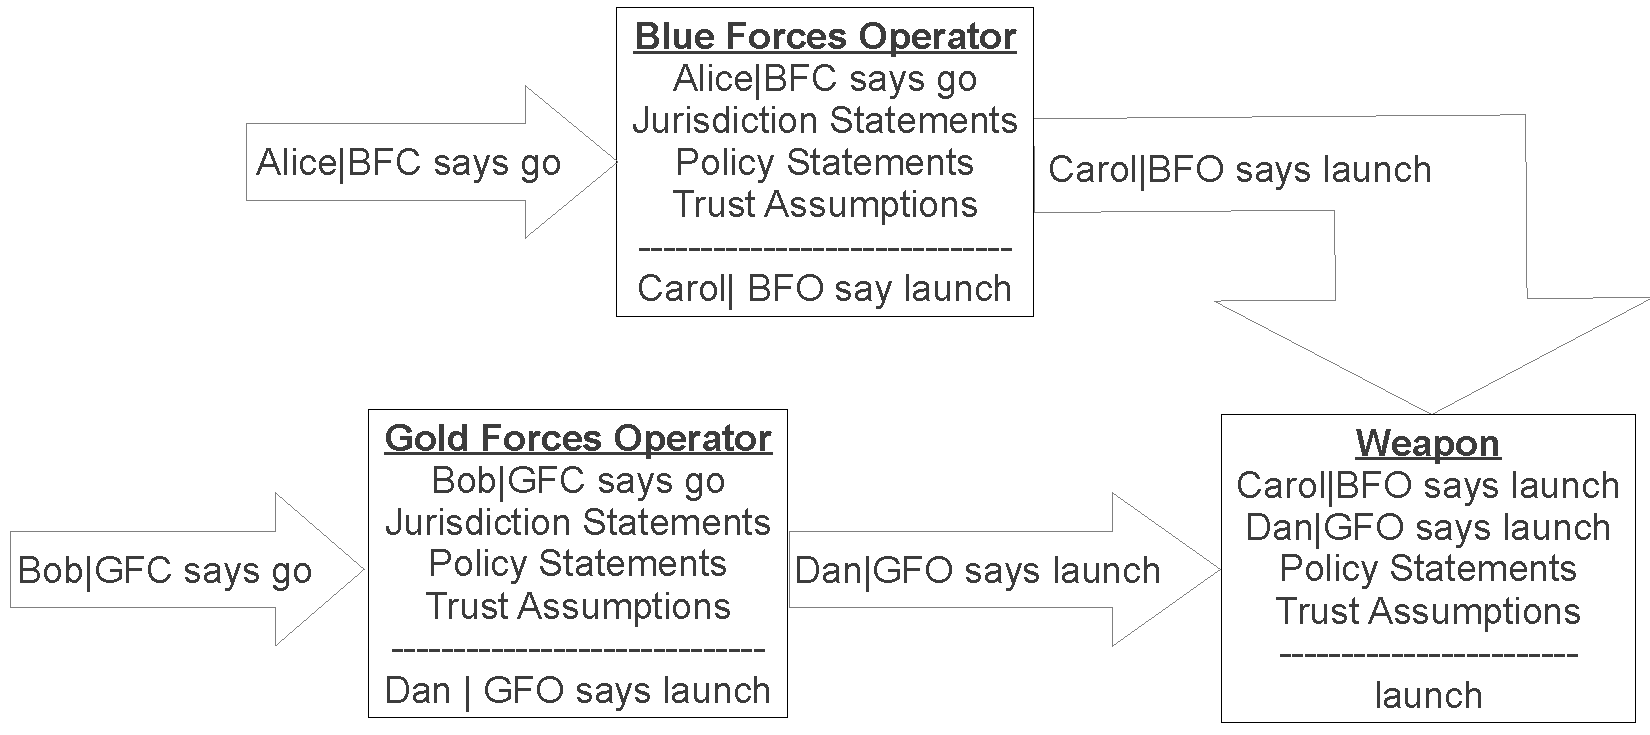
\includegraphics[width=0.95\linewidth]{Figures/c2conops/launchCONOPSRefine1}}
    \end{minipage}
    &
    \begin{minipage}{0.48\linewidth}
      \centering{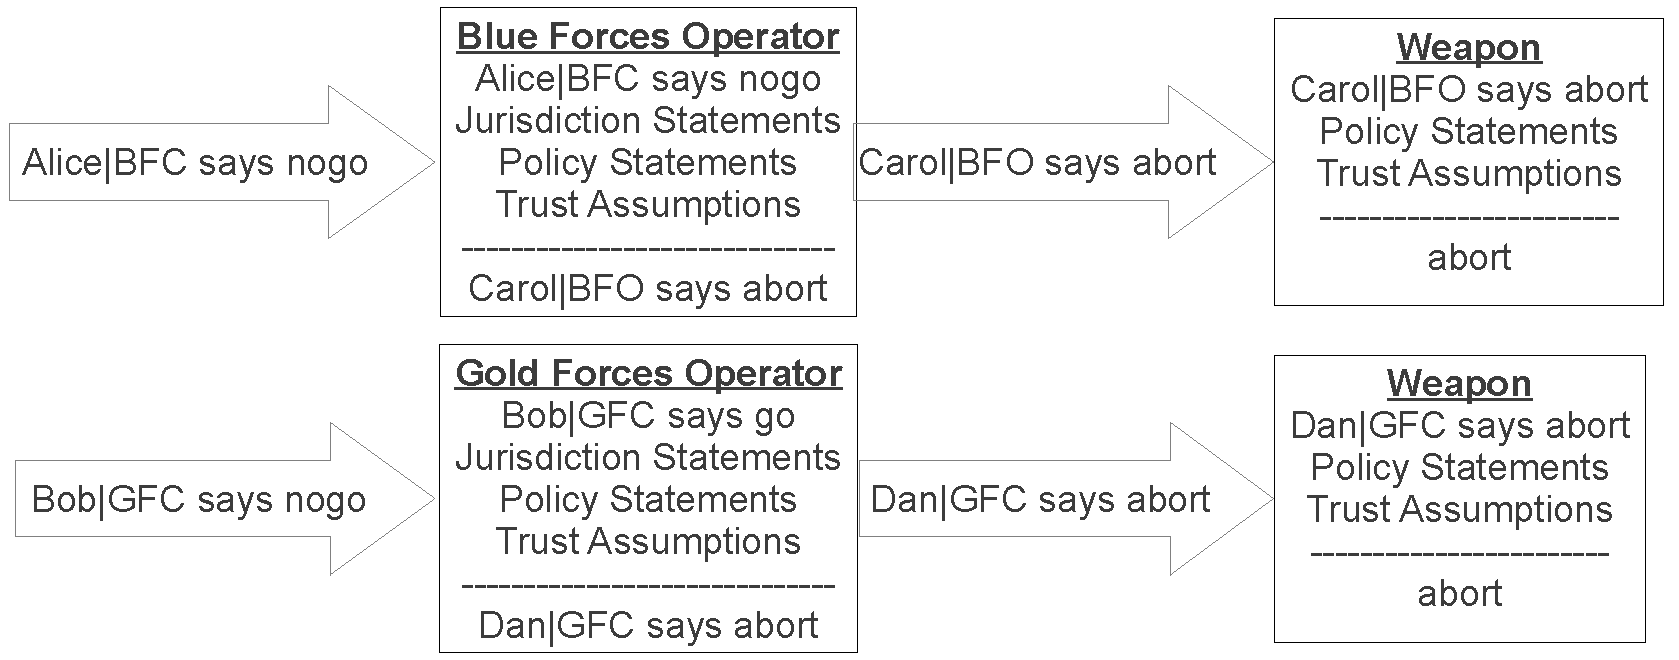
\includegraphics[width=0.95\linewidth]{Figures/c2conops/abortCONOPSRefine1}}
    \end{minipage}\\
    (a) Launch CONOPS & (b) Abort CONOPS\\
  \end{tabular}
  
  \caption{Launch and Abort CONOPS with Assigned Personnel}
  \label{fig:conops-with-people}
\end{figure}

The first refinement to the high-level CONOPS expressed only in terms
of mission roles is to add the notion of authentication of principals
acting in mission roles. A principal $P$ acting in a mission role
\emph{Role} giving command $\varphi$ is represented by $P \quoting
Role \says \varphi$. If \emph{P's} authority to act in role
\emph{Role} is recognized, i.e., $\reps{P}{Role}{\varphi}$, and if
$Role \controls \varphi$, then we conclude $\varphi$ is justified,
from the \emph{Reps} inference rule shown below:
\begin{gather*}
  \irule
  {Q \controls \varphi \quad \reps{P}{Q}{\varphi} \quad 
   P \quoting Q \says \varphi}
  {\varphi}
  {Reps}.
\end{gather*}
Figure~\ref{fig:conops-with-people} is a block diagram that refines
the high-level launch and abort CONOPS in
Figure~\ref{fig:launch-abort-conops}.  The primary differences are in
the messages sent among principals. Instead of mission roles speaking,
principals claiming to be acting in mission roles make
statements. Figure~\ref{fig:conops-with-people} shows Alice acting as
Blue Forces Commander, Bob acting as Gold Forces Commander, Carol
acting as Blue Forces Operator, and Dan acting as Gold Forces
Operator.

We recall that Blue and Gold Forces Commanders have the authority to
assign personnel to the roles of Blue and Gold Operators,
respectively:
\begin{gather*}
  BFC \controls (\reps{P}{BFO}{\varphi})\\
  GFC \controls (\reps{P}{GFO}{\varphi}).
\end{gather*}
Table~\ref{tab:roles-authority} gives a complete listing of roles and
their associated authority. Table~\ref{tab:role-assignments} shows the
personnel assignments to mission roles and who authenticates them.
Notice that authorizations for personnel designated as Blue and Gold
Forces Commanders are designated as \emph{pre-distributed prior to
  mission}. This is similar to the case where the cryptographic key of
a root certificate authority is pre-loaded into computers. In this
CONOPS, mission equipment and weapons must be loaded with
\emph{roots of trust} prior to the start of the mission. In this
case, it will include the personnel who are authorized as commanders
as well as cryptographic keys of root authorities. \emph{The loading
  of this information must be done with the utmost integrity and
  security otherwise all is lost.}

\paragraph*{Derived Inference Rules}
\label{sec:deriv-infer-rules}

We now refine the derived inference rules corresponding to BFO Launch,
GFO Launch, BFO Abort, GFO Abort, and when the weapon is launched or
aborted.

\subparagraph{BFO and GFO Launch}
\label{sec:bfo-gfo-launch}

% \begin{table}[t]
%   \centering
%   \begin{footnotesize}
%     \begin{tabular}{|r<{.}>{$}l<{$}l|}
%       \hline
%       1 & Q \controls \varphi_1 & Assumption, jurisdiction of Q\\
%       2 & \reps{P}{Q}{\varphi} & P acting in role of Q\\
%       3 & P \quoting Q \says \varphi_1 & Command from P\\
%       4 & \varphi_1 \implies \varphi_2 & Policy statement\\
%       5 & \varphi_1 & 1, 2, 3 Reps\\
%       6 & \varphi_2 & 5, 4 Modus Ponens\\
%       7 & R \says \varphi_2 & 6 Says\\
%       \hline
%     \end{tabular}
%   \end{footnotesize}

%   \caption{Proof of Implied Controls with Delegation}
%   \label{tab:delegation-proof}
% \end{table}
Based on Figure~\ref{fig:conops-with-people} we refine the derived
inference rules \emph{BFO Launch} and \emph{GFO Launch} based on the
form of received orders and the trust assumptions and policy
statements needed by operators to issue the launch command to the
weapon.

As we are using delegation of principals to mission roles as a means
for assigning people to mission roles, our launch rules for operators
require operators to know who is operating in the role of Blue or Gold
Forces Commander. This knowledge is reflected in the statements
$\reps{Alice}{BFC}{\action{go}}$ and $\reps{Bob}{GFC}{\action{go}}$.

\begin{footnotesize}
  \begin{gather*}
    \irule {
      \begin{array}{c}
        BFC \controls \action{go} \quad Alice \quoting BFC \says \action{go} \quad 
        \reps{Alice}{BFC}{\action{go}} \quad \action{go} \implies \action{launch}
      \end{array}
    } {Carol \quoting BFO \says \action{launch}}
    {BFO Launch 2} \\
    \irule {
      \begin{array}{c}
        GFC \controls \action{go} \quad Bob \quoting GFC \says \action{go} \quad 
        \reps{Bob}{GFC}{\action{go}} \quad \action{go} \implies \action{launch}
      \end{array}
    } {Dan \quoting GFO \says \action{launch}} {GFO Launch 2}
  \end{gather*}
\end{footnotesize}

We see that as before both of the Launch rules are instances of the
same rule:

\begin{footnotesize}
  \begin{gather*}
    \irule {\begin{array}{c} R_1 \controls \varphi_1 \quad
       P_1 \quoting R_1 \says \varphi_1 \quad \reps{P_1}{R_1}{\varphi_1} 
        \quad \varphi_1 \implies \varphi_2
      \end{array}
    } {P_2 \quoting R_2 \says \varphi_2} {Delegates}
  \end{gather*}
\end{footnotesize}

\subparagraph*{BFO and GFO Abort}

Left as an exercise.
%% % HERE ARE THE SPECIFIC RULES
% \begin{footnotesize}
%   \begin{gather*}
%     \irule {
%       \begin{array}{c}
%         BFC \controls \action{nogo} \quad \reps{Alice}{BFC}{\action{nogo}} \quad Alice \quoting BFC \says \action{nogo} \quad
%         \action{nogo} \implies \action{abort}
%       \end{array}
%     } {BFO \says \action{abort}}
%     {BFO Abort 2}\\
%     \irule {
%       \begin{array}{c}
%         GFC \controls \action{nogo} \quad \reps{Bob}{GFC}{\action{nogo}} \quad Bob \quoting GFC \says \action{nogo} \quad
%         \action{nogo} \implies \action{abort}
%       \end{array}
%     } {GFO \says \action{abort}} {GFO Abort 2}
%   \end{gather*}
% \end{footnotesize}

\subparagraph*{Weapons Launch}

\begin{footnotesize}
  \begin{gather*}
    \irule {
      \begin{array}[h]{c}
        BFO \with GFO \controls \action{launch} \quad Carol \quoting BFO \says \action{launch} \quad Dan\quoting GFO \says \action{launch} \\
        \reps{Carol}{BFO}{\action{launch}} \quad \reps{Dan}{GFO}{\action{launch}}
      \end{array}
    } {\action{launch}} {Weapons Launch 2}
  \end{gather*}
\end{footnotesize}

\subparagraph*{Weapons Abort}

Left as an exercise.

% \begin{exercise}[\synthesis]
% Consider the following inference rule and its definition (already defined
%     in \emph{missioninf\_rules.sml}).
% \begin{scriptsize}
% \begin{lstlisting}
% (***********************************************************
% * ImpliedControlsDelegation
% *
% * ImpliedControlsDelegation : term -> thm -> thm -> thm -> thm -> thm
% *
% * SYNOPSIS
% * Deduces formula f2 if the principal who says f1, controls f1, and
% * f1 impf f2.
% *
% * DESCRIPTION
% *
% *     A1 |- (M,Oi,Os) sat Q controls f1  A2 |- (M,Oi,Os) sat reps P Q f1
% *            A3 |- P quoting Q says f1  A4 |- f1 impf f2
% *     ------------------------------------------------------- ImpliedControlsDelegation R
% *          A1 u A2 u A3 u A4 |- (M,Oi,Os) sat R says f2
% *
% * FAILURE
% * Fails unless the theorems match in terms of principals and formulas
% * in the access-control logic.
% ***********************************************************)
% fun ImpliedControlsDelegation R th1 th2 th3 th4 =
% MATCH_MP
% (MATCH_MP 
%  (MATCH_MP 
%   (MATCH_MP (ISPEC R ImpliedControlsDelegation_thm) th1) th2) th3) th4;  
% \end{lstlisting}
% \end{scriptsize}
%   \begin{enumerate}[{A.}]
%   \item Prove in HOL the \emph{BFO\_Launch} theorem using the
%     \emph{ImpliedControlsDelegation} inference rule.
%   \item Prove in HOL the \emph{GFO\_Launch} theorem using the
%     \emph{ImpliedControlsDelegation} inference rule.
%   \end{enumerate}
% \end{exercise}

\begin{exercise}[\synthesis]
  For BFO and GFO launch, do the following:
  \begin{enumerate}[{A.}]
  \item Prove their underlying theorems in HOL.
  \item Devise ML inference rules based on their theorems.
  \end{enumerate}
\end{exercise}

\begin{exercise}[\synthesis]
  For BFO and GFO abort, do the following:
  \begin{enumerate}[{A.}]
  \item Prove their underlying theorems in HOL.
  \item Devise ML inference rules based on their theorems.
  \end{enumerate}
\end{exercise}

\begin{exercise}[\synthesis]
  For weapons launch, do the following:
  \begin{enumerate}[{A.}]
  \item Prove its underlying theorem in HOL.
  \item Devise an ML inference rule based on the theorem.
  \end{enumerate}
\end{exercise}

\begin{exercise}[\synthesis]
  For weapons abort, do the following:
  \begin{enumerate}[{A.}]
  \item Prove its underlying theorem in HOL.
  \item Devise an ML inference rule based on its theorem.
  \end{enumerate}
\end{exercise}


\section{Refinement 3: CONOPS with Key and Role Certificates}
\label{sec:refinement3}

\begin{figure}[t]
  \centering
  \begin{tabular}{cc}
  \begin{minipage}{0.45\linewidth}
    \begin{center}
      \begin{scriptsize}
        \begin{tabular}{|r|l|}
          \hline
          \multicolumn{2}{|c|}{Key Certificate}\\
          \hline
          Issuer & Certificate Authority\\
          \hline
          Principal Name & $P$\\
          \hline
          Cryptographic Key & $K_P$\\
          \hline
          Digital signature & $K_{CA} \says (K_P \speaksfor P)$\\
          \hline
        \end{tabular}
      \end{scriptsize}
    \end{center}

  \end{minipage}
  &
  \begin{minipage}{0.45\linewidth}
    \begin{center}
      \begin{scriptsize}
        \begin{tabular}{|r|l|}
          \hline
          \multicolumn{2}{|c|}{Role Certificate}\\
          \hline
          Issuer & Role Authority\\
          \hline
          Principal Name & $P$\\
          \hline
          Role & $Role$\\
          \hline
          Jurisdiction & $\varphi_1 \ldots \varphi_n$\\
          \hline
          Digital signature & $K_{RA} \says (\reps{P}{Role}{\varphi_i})$\\
          \hline
        \end{tabular}
      \end{scriptsize}
    \end{center}
  \end{minipage}\\
  (a) Key Certificate & (b) Role Certificate
\end{tabular}
  \caption{Key and Role Certificates}
  \label{fig:key-role-certs}
\end{figure}

\begin{figure}[t]
  \centering
  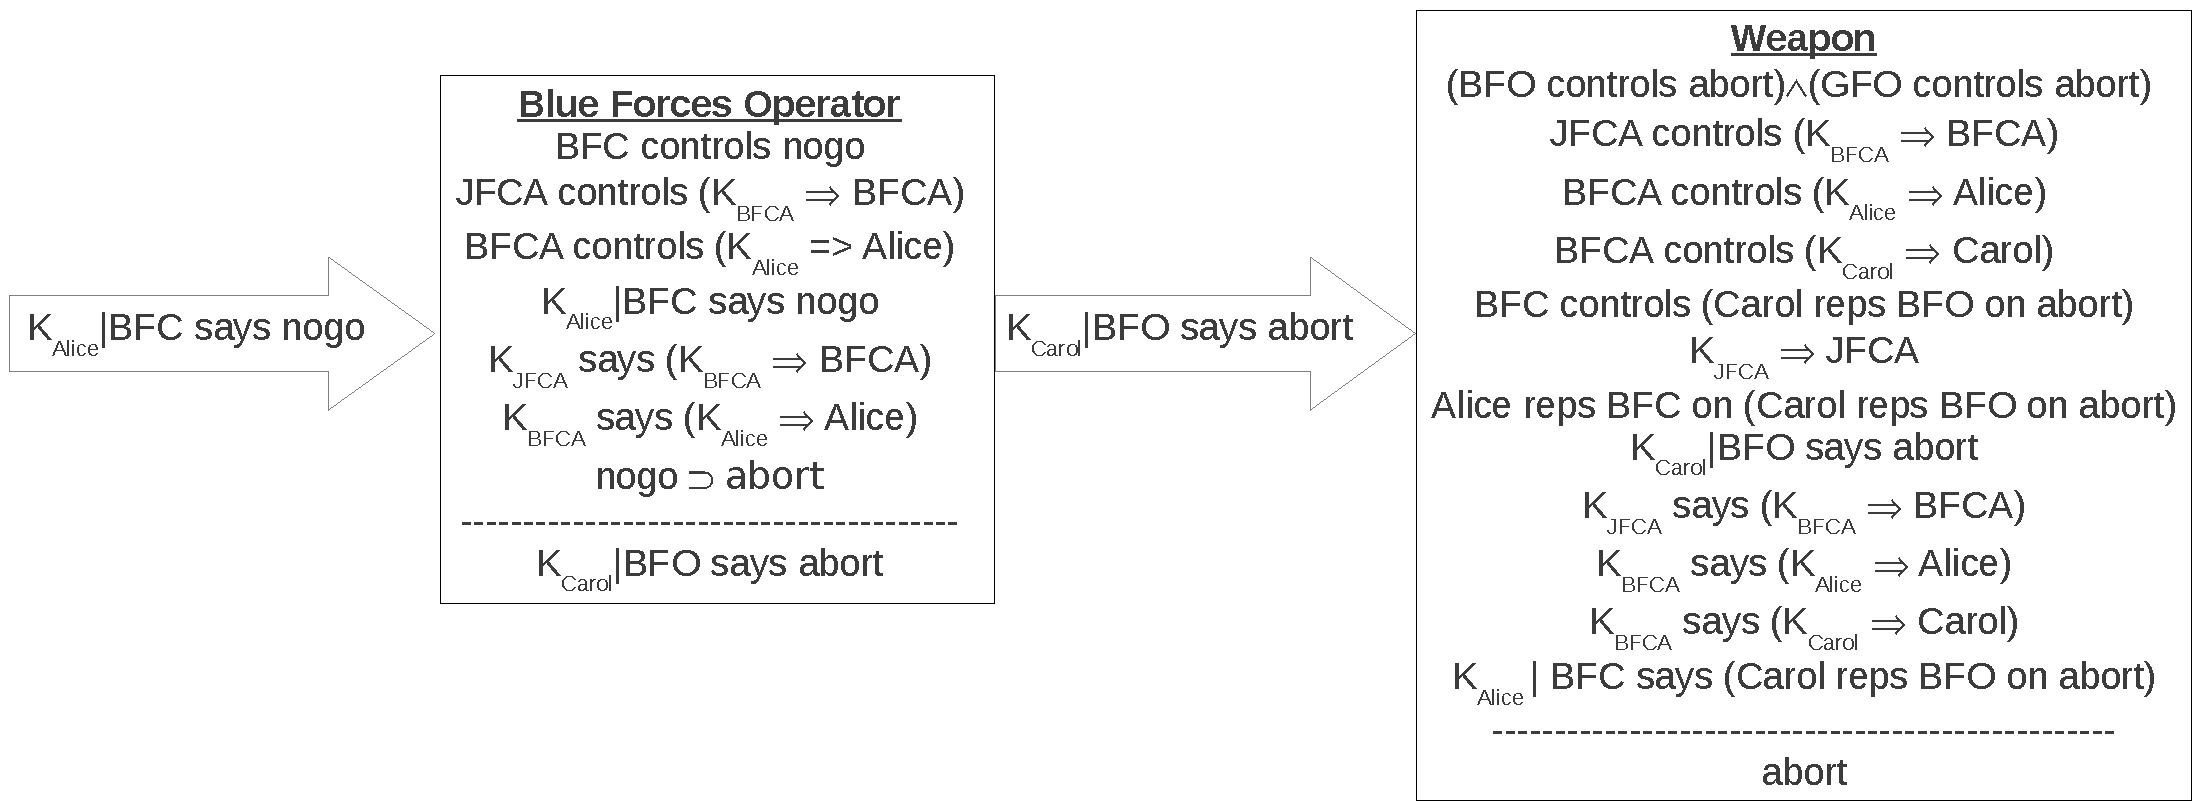
\includegraphics[width=0.9\linewidth]{Figures/c2conops/abortCONOPSRefine3}
  \caption{Weapons Abort from BFC with Keys and Authorizations}
  \label{fig:abort-refinement3}
\end{figure}

\begin{figure}[t]
  \centering
  \begin{footnotesize}
    \begin{tabular}{r<{.}>{$}p{0.55\linewidth}<{$}p{0.4\linewidth}}
      1 & (BFO \controls \action{abort}) \wedge (GFO \controls \action{abort}) & Jurisdiction assumption\\
      2 & JFCA \controls (K_{BFCA} \speaksfor BFCA) & Jurisdiction assumption\\
      3 & BFCA \controls (K_{Alice} \speaksfor Alice) & Jurisdiction assumption\\
      4 & BFCA \controls (K_{Carol} \speaksfor Carol) & Jurisdiction assumption\\
      5 & BFC \controls (\reps {Carol}{BFO}{\action{abort}}) & Jurisdiction assumption\\
      6 & K_{JFCA} \speaksfor JFCA & Trust assumption\\
      7 & \reps{Alice}{BFC}{\reps {Carol}{BFO}{\action{abort}}} & Trust assumption\\
      8 & K_{Carol} \quoting BFO \says \action{abort} & Input command\\
      9 & K_{JFCA} \says (K_{BFCA} \speaksfor BFCA) & Key certificate\\
      10 & K_{BFCA} \says (K_{Alice} \speaksfor Alice) & Key certificate\\
      11 & K_{BFCA} \says (K_{Carol} \speaksfor Carol) & Key certificate\\
      12 & K_{Alice} \quoting BFC \says (\reps{Carol}{BFO}{\action{abort}}) & Role certificate\\
      13 & JFCA \says (K_{BFCA} \speaksfor BFCA) & 6, 9 Derived Speaks For\\
      14 & K_{BFCA} \speaksfor BFCA & 2, 13 Controls\\
      15 & BFCA \says (K_{Alice} \speaksfor Alice) & 14, 10 Derived Speaks For\\
      16 & K_{Alice} \speaksfor Alice & 3, 15 Controls\\
      17 & BFCA \says (K_{Carol} \speaksfor Carol) & 14, 11 Derived Speaks For\\
      18 & K_{Carol} \speaksfor Carol & 4, 17 Controls\\
      19 & BFC \speaksfor BFC & Idempotency of $\speaksfor$\\
      20 & K_{Alice} \quoting BFC \speaksfor Alice \quoting BFC & 16, 19 Monotonicity of $\speaksfor$\\
      21 & Alice \quoting BFC \says (\reps{Carol}{BFO}{\action{abort}}) & 20, 12 Derived Speaks For\\
      22 & BFO \speaksfor BFO & Idempotency of $\speaksfor$\\
      23 & K_{Carol} \quoting BFO \speaksfor Carol \quoting BFO & 18, 22 Monotonicity of $\speaksfor$\\
      24 & Carol \quoting BFO \says \action{abort} & 23, 8 Derived Speaks For\\
      25 & \reps{Carol}{BFO}{\action{abort}} & 5, 7, 21 Reps\\
      26 & BFO \controls \action{abort} & 1 Simplification (1)\\
      27 & \action{abort} & 26, 25, 24 Reps\\
    \end{tabular}
  \end{footnotesize}

  \caption{Proof of AlternateControlsRepsKey1}
  \label{fig:alternate-controls-reps-key1}
\end{figure}
Our next refinement adds details on the use of cryptographic keys,
public-key certificates, and certificates of role authorizations. In
Refinement 2, we have people in roles giving orders, e.g., $Carol
\quoting BFO \says \action{abort}$.

In Refinement 3, we have orders in the form of cryptographically
signed statements, e.g., $K_{Carol} \quoting BFO \says
\action{abort}$. Our objective, if we are the weapon receiving Carol's
signed order to abort is to conclude that we have received a
legitimate actionable order from a Blue Force Operator.  This
requires the following be established:
\begin{enumerate}
\item $K_{Carol}$ is in fact Carol's key,
\item if we determine Carol issued the order, that Carol
  is a Blue Force Operator, and
\item as in Refinement 2, that her order as Blue Force Operator falls
  within her purview.
\end{enumerate}

To determine the above, we need additional infrastructure in the form
of certificates (digitally signed statements from trusted
authorities), i.e., additional \emph{trust infrastructure}. An
informal description of the distribution of authority for
authenticating key associations and assignment of mission roles to
mission staff is given in Tables~\ref{tab:mission-ca} and
\ref{tab:roles-authority}, which specify the structure of public-key
certificate authorities (JFCA, BFCA, and GFCA) and the authority of
Blue and Gold Force Commanders to authorize their respective mission
staff as Operators.

The additional trust infrastructure for key and role assignments is in
the form of key and role certificates, as shown in
Figure~\ref{fig:key-role-certs}. Figure~\ref{fig:abort-refinement3}
shows the inference rule used by the weapon to conclude that it should
abort when receiving an \emph{abort} command from Carol as Blue Force
Operator.

Figure~\ref{fig:alternate-controls-reps-key1} is a proof of the
\emph{AlternateControlsRepsKey1} rule shown in
Figure~\ref{fig:abort-refinement3}. The specific certificates we need
are as follows:
\begin{align*}
  K_{JFCA} & \says (K_{BFCA} \speaksfor BFCA)\\
  K_{BFCA} & \says (K_{Alice} \speaksfor Alice)\\
  K_{BFCA} & \says (K_{Carol} \speaksfor Carol)\\
  K_{Alice} \quoting BFC & \says (\reps{Carol}{BFO}{abort})\\
\end{align*}
The first three certificates are public-key certificates. The last
certificate is a \emph{role certificate} signed by Alice as BFC
certifying that Carol is a Blue Force Operator.

With both signed key and role certificates, ultimately, there are
trust assumptions corresponding to root keys and root roles. In this
scenario, the root key and role are (1) the key associated with JFCA,
and (2) the role BFC. As these are the highest authorities on keys and
mission roles, there are no higher authorities to vouch for
them. Thus, the keys and personnel associated with them must be
installed prior to the mission start under carefully controlled
circumstances.

There are six jurisdiction assumptions (statements 1 through 6 in
Figure~\ref{fig:alternate-controls-reps-key1}). These are presumably
``hard-wired'' into to weapon's control system.

The corresponding general theorem in HOL appears below.

\begin{quote}
  \tealtext{[AlternateControlRepsKey1]}
  \HOLcTwoDrulesTheoremsAlternateControlRepsKeyOne
\end{quote}


There are five remaining operations: BFO Launch, GFO Launch, GFO
abort, Weapon Launch, and Weapon GFO Abort. They are developed in much
the same way as illustated by our development of Weapon BFO Abort,
here.


% ---- this points LaTeX to book.tex ---- 
% Local Variables: 
% TeX-master: "book"
% End:

%  LocalWords:  CGs criticality BFCAs GFCAs JFCAs JFCA's Modus Ponens
%  LocalWords:  missionCommands weaponCommands missionRoles thm ACL
%  LocalWords:  missionStaff missionCONOPS commandTheory DualControl
%  LocalWords:  AlternateControls ImpliedControlsSays DualControls RL
%  LocalWords:  missionRolesTheory ImpliedControlsDelegation ASSUM th
%  LocalWords:  impf AltControls andf GF missioninf ISPEC
%  LocalWords:  missionKeysTheory
